\documentclass[landscape,a4paper]{article}
\usepackage{xeCJK}
\usepackage{setspace}%使用间距宏包
\usepackage{listings}
\usepackage{geometry}
\usepackage{multicol} %用于实现在同一页中实现不同的分栏
\usepackage{amsthm}
\usepackage{amsmath}
\usepackage{amssymb}
\usepackage{harpoon}
\usepackage{bm}
\geometry{left=0.5cm,right=0.5cm,top=0.5cm,bottom=1.2cm}
\usepackage{mathrsfs} %支持花体字母
\lstset{breaklines}%自动将长的代码行换行排版
\lstset{extendedchars=false}%解决代码跨页时,章节标题,页眉等汉.2字不显示的问题
\usepackage{color}
\usepackage{xcolor}
\definecolor{keywordcolor}{rgb}{0, 0, 0}

\setmainfont{Courier} 

\usepackage{listings}
\lstset{breaklines}%这条命令可以让LaTeX自动将长的代码行换行排版
\lstset{extendedchars=false}%这一条命令可以解决代码跨页时,章节标题,页眉等汉字不显示的问题
\lstset{language=C++, %用于设置语言为C++
	keywordstyle=\color{keywordcolor} \bfseries,
	identifierstyle=,
	basicstyle=\ttfamily,
	commentstyle=\color{black} \textit,
	stringstyle=\ttfamily,
	showstringspaces=false,
	tabsize=2,
	frame=single, %边框
	captionpos=b
}
\newcommand{\stlf}[2]{\genfrac{ [ }{ ] }{0pt}{}{#1}{#2}}
\newcommand{\stls}[2]{\genfrac{ \{ }{ \} }{0pt}{}{#1}{#2}}

\usepackage{titlesec}
\titleformat{\section}
{\normalfont\scriptsize\bfseries}{\thesection}{1em}{}
\titleformat{\subsection}
{\normalfont\scriptsize\bfseries}{\thesubsection}{1em}{}
\titleformat{\subsubsection}
{\normalfont\scriptsize\bfseries}{\thesubsubsection}{1em}{}
\titleformat{\paragraph}[runin]
{\normalfont\scriptsize\bfseries}{\theparagraph}{1em}{}
\titleformat{\subparagraph}[runin]
{\normalfont\scriptsize\bfseries}{\thesubparagraph}{1em}{}
\titlespacing*{\subsubsection}{0pt}{0pt}{0pt}
\titlespacing*{\subsection}{0pt}{0pt}{0pt}
\titlespacing*{\section}{0pt}{0pt}{0pt}



	\title{Metis}
\begin{document}\scriptsize
\begin{titlepage}

\newcommand{\HRule}{\rule{\linewidth}{0.5mm}}
\center
\textsc{\LARGE Templates}\\[1.5cm] 
\textsc{\Large Shanghai Jiaotong University}\\[0.5cm]
%\textsc{\large ACM Class}\\[0.5cm]
\HRule \\[0.4cm]
{ \huge \bfseries Metis}\\[0.4cm] 
\HRule \\[1.5cm]

\begin{minipage}{0.4\textwidth}
\begin{flushleft} \large
\emph{Member:}\\
 \textsc{Sishan Long \\ Yutong Xie \\ Jingyi Cai}
\end{flushleft}
\end{minipage}
~
\begin{minipage}{0.4\textwidth}
\begin{flushright} \large
\emph{Coach:} \\
\textsc{Yunqi Li \\ Xueyuan Zhao}
\end{flushright}
\end{minipage}\\[4cm]


%{\large \today}\\[3cm] 
%\includegraphics{frontpage.jpeg}

\vfill

\end{titlepage}
	
	
	
	\begin{spacing}{0.3}	
	%\columnseprule=0.5pt
	\begin{multicols}{2}
	
	\tableofcontents
	
	\subsubsection{开栈}
\begin{lstlisting}[language=C++]
#pragma comment(linker, “/STACK:16777216”)//大小随便定
\end{lstlisting}
\subsection{运行命令}
\begin{lstlisting}[language=C++]
g++ A.cpp -o A -Wall -O2
\end{lstlisting}
	
\section{计算几何}

\subsection{精度}
\begin{lstlisting}[language=C++]
const double eps = 1e-8, pi = acos(-1.0);
inline int sign(double x) {return x < -eps ? -1 : x > eps;}
inline double Acos(double x) {
	if (sign(x + 1) == 0) return acos(-1.0);
	if (sign(x - 1) == 0) return acos(1.0);
	return acos(x);
}
inline double Asin(double x) {
	if (sign(x + 1) == 0) return asin(-1.0);
	if (sign(x - 1) == 0) return asin(1.0);
	return asin(x);
}
inline double Sqrt(double x) {
	if (sign(x) == 0) return 0;
	return sqrt(x);
}
\end{lstlisting}
\subsection{点类(向量类)}
\begin{lstlisting}[language=C++]
struct point
{
	double x,y;
	point(){}
	point(double x,double y) : x(x), y(y) {}
	double len() const {return(sqrt(x * x + y * y));}
	point unit() const {double t = len(); return(point(x / t, y / t));}
	point rotate() const {return(point(-y, x));}
	point rotate(double t) const
        {return(point(x*cos(t)-y*sin(t), x*sin(t)+y*cos(t)));}
};
point operator +(const point &a, const point &b)
    {return(point(a.x + b.x, a.y + b.y));}
point operator -(const point &a, const point &b)
    {return(point(a.x - b.x, a.y - b.y));}
point operator *(const point &a, double b)
    {return(point(a.x * b, a.y * b));}
point operator /(const point &a, double b)
    {return(point(a.x / b, a.y / b));}
bool operator <(const point &a, const point &b)
    {return(sign(a.x - b.x)<0||sign(a.x - b.x)==0&&sign(a.y - b.y)<0);}
double dot(const point &a, const point &b)
    {return(a.x * b.x + a.y * b.y);}
double det(const point &a, const point &b)
    {return(a.x * b.y - a.y * b.x);}
double mix(const point &a, const point &b, const point &c) 
    {return dot(det(a, b), c);}//混合积,它等于四面体有向体积的六倍
double dist(const point &a, const point &b)
    {return((a - b).len());}
\end{lstlisting}
\subsection{直线}
\begin{lstlisting}[language=C++]
//点在直线的哪一侧
int side(const point &p, const point &a, const point &b)
    {return(sign(det(b - a, p - a)));}
//点是否在线段上
bool online(const point&p,const point&a,const point&b)
    {return(sign(dot(p - a, p - b ))<=0 && sign(det(p - a, p - b))==0);}
//点关于直线垂线交点
point project(const point &p,const point &a, const point &b){
    double t = dot(p - a, b - a) / dot(b - a, b - a);
    return(a + (b - a) * t);}
//点到直线距离
double ptoline(const point &p, const point &a, const point &b)
    {return(fabs(det(p - a, p - b)) / dist(a, b));}
//点关于直线的对称点
point reflect(const point &p, const point &a, const point &b)
    {return(project(p, a, b) * 2 - p);}
//判断两直线是否平行
bool parallel(const point &a,const point &b,const point &c,const point &d)
    {return(sign(det(b - a, d - c)) == 0);}
//判断两直线是否垂直
bool orthogonal(const point&a,const point&b,const point&c,const point&d)
    {return(sign(dot(b - a, d - c)) == 0);}
//判断两线段是否相交
bool cross(const point&a,const point&b,const point&c,const point&d)
    {return(side(a, c, d) * side(b, c, d) == -1 && side(c, a, b) * side(d, a, b) == -1);}
//求两线段的交点
point intersect(const point&a,const point&b,const point&c,const point&d){
    double s1 = det(b - a, c - a), s2 = det(b - a, d - a);
    return((c * s2 - d * s1) / (s2 - s1));}
//两点求线ax+by+c=0
line point_make_line(point a, point b) {
     line h; h.a = b.y - a.y; h.b = -(b.x - a.x); h.c = -a.x * b.y + a.y * b.x;
     return h;
}
//线段平移D的长度
line move_d(line a, const double d) {
	return line(a.a, a.b, a.c + d * sqrt(a.a * a.a + a.b * a.b);
}
\end{lstlisting}
\subsection{圆}
\begin{lstlisting}[language=C++]
//直线与圆交点
pair <point,point> intersect(const point &a,const point &b,const point &o,double r){
    point tmp = project(o, a, b); double d = dist(tmp, o);
    double l = Sqrt(sqr(r) - sqr(d));
    point dir = (b - a).unit() * l;
    return(make_pair(tmp + dir, tmp - dir));}
//两圆交点
pair <point, point> intersect(const point &o1, double r1,const point &o2, double r2){
    double d = dist(o1, o2), x = (sqr(r1) - sqr(r2)) / (2 * d) + d / 2;
    double l = Sqrt(sqr(r1) - sqr(x)); point dir = (o2 - o1).unit();
    return(make_pair(o1 + dir * x + dir.rotate() * l,
                     o1 + dir * x - dir.rotate() * l));}
//点与圆切线与圆交点
point tangent(const point &p, const point &o, double r)
    {return(intersect((p + o) / 2, dist(p, o) / 2, o, r).first);}
//两圆内公切线
pair <point,point> intangent(const point &o1,double r1,const point &o2,double r2){
    double t = r1 / (r1 + r2); point tmp = o1 + (o2 - o1) * t;
    point P = tangent(tmp, o1, r1), Q = tangent(tmp, o2, r2);
    return(make_pair(P, Q));}
//两圆外公切线
pair <point,point> extangent(const point &a, double r1,const point &b, double r2){
    if (sign(r1 - r2) == 0) {
        point dir = (b - a).rotate().unit();
        return(make_pair(a + dir * r1, b + dir * r2));}
    if (sign(r1 - r2) > 0) {
		pair <point, point> tmp = extangent(b, r2, a, r1);
        return(make_pair(tmp.second, tmp.first));}
    point p = tangent(a, b, r2 - r1), dir = (p - b).unit();
    return(make_pair(a + dir * r1, b + dir * r2));}
//两圆交线|P - P1| = r1 and |P - P2| = r2 of the ax + by + c = 0 form
void CommonAxis(point p1, double r1, point p2, double r2, double &a, double &b, double &c) {
	double sx = p2.x + p1.x, mx = p2.x - p1.x;
	double sy = p2.y + p1.y, my = p2.y - p1.y;
	a = 2 * mx; b = 2 * my; c = -sx * mx – sy * my – (r1 + r2) * (r1 - r2);
}
//两圆交点,两个圆不能共圆心,请特判
int CircleCrossCircle(point p1, double r1, point p2, double r2, point &cp1, point &cp2) {
	double mx = p2.x - p1.x, sx = p2.x + p1.x, mx2 = mx * mx;
	double my = p2.y - p1.y, sy = p2.y + p1.y, my2 = my * my;
	double sq = mx2 + my2, d = -(sq – sqr(r1 - r2)) * (sq – sqr(r1 + r2));
	if (d + eps < 0) return 0; if (d < eps) d = 0; else d = sqrt(d);
	double x = mx * ((r1 + r2) * (r1 - r2) + mx * sx) + sx * my2;
	double y = my * ((r1 + r2) * (r1 - r2) + my * sy) + sy * mx2;
	double dx = mx * d, dy = my * d; sq *= 2;
	cp1.x = (x - dy) / sq; cp1.y = (y + dx) / sq;
	cp2.x = (x + dy) / sq; cp2.y = (y - dx) / sq;
	if (d > eps) return 2; else return 1;
}
//两圆面积交:dist是距离,dis是平方
double twoCircleAreaUnion(point a, point b, double r1, double r2) {
	if (r1 + r2 <= (a - b).dist()) return 0;
	if (r1 + (a – b).dist() <= r2) return pi * r1 * r1;
	if (r2 + (a – b).dist() <= r1) return pi * r2 * r2;
	double c1, c2, ans = 0;
	c1 = (r1 * r1 – r2 * r2 + (a – b).dis()) / (a – b).dist() / r1 / 2.0;
	c2 = (r2 * r2 - r1 * r1 + (a – b).dis()) / (a – b).dist() / r2 / 2.0;
	double s1, s2; s1 = acos(c1); s2 = acos(c2);
	ans += s1 * r1 * r1 – r1 * r1 * sin(s1) * cos(s1);
	ans += s2 * r2 * r2 – r2 * r2 * sin(s2) * cos(s2);
	return ans;
}
\end{lstlisting}
\subsubsection{最小覆盖球}
\begin{lstlisting}
double eps(1e-8);
int sign(const double & x) { return (x > eps) - (x + eps < 0);}
bool equal(const double & x, const double & y) {return x + eps > y and y + eps > x;}
struct Point {
	double x, y, z;
	Point() {}
	Point(const double & x, const double & y, const double & z) : x(x), y(y), z(z){}
	void scan() {scanf("%lf%lf%lf", &x, &y, &z);}
	double sqrlen() const {return x * x + y * y + z * z;}
	double len() const {return sqrt(sqrlen());}
	void print() const {printf("(%lf %lf %lf)\n", x, y, z);}
} a[33];
Point operator + (const Point & a, const Point & b) {return Point(a.x + b.x, a.y + b.y, a.z + b.z);}
Point operator - (const Point & a, const Point & b) {return Point(a.x - b.x, a.y - b.y, a.z - b.z);}
Point operator * (const double & x, const Point & a) {return Point(x * a.x, x * a.y, x * a.z);}
double operator % (const Point & a, const Point & b) {return a.x * b.x + a.y * b.y + a.z * b.z;}
Point operator * (const Point & a, const Point & b) {return Point(a.y * b.z - a.z * b.y, a.z * b.x - a.x * b.z, a.x * b.y - a.y * b.x);}
struct Circle {
	double r; Point o;
	Circle() {o.x = o.y = o.z = r = 0;}
	Circle(const Point & o, const double & r) : o(o), r(r) {}
	void scan() {o.scan();scanf("%lf", &r);}
	void print() const {o.print();printf("%lf\n", r);}
};
struct Plane {
	Point nor; double m;
	Plane(const Point & nor, const Point & a) : nor(nor){m = nor % a;}
};
Point intersect(const Plane & a, const Plane & b, const Plane & c) {
	Point c1(a.nor.x, b.nor.x, c.nor.x), c2(a.nor.y, b.nor.y, c.nor.y), c3(a.nor.z, b.nor.z, c.nor.z), c4(a.m, b.m, c.m);
	return 1 / ((c1 * c2) % c3) * Point((c4 * c2) % c3, (c1 * c4) % c3, (c1 * c2) % c4);
}
bool in(const Point & a, const Circle & b) {return sign((a - b.o).len() - b.r) <= 0;}	
bool operator < (const Point & a, const Point & b) {
	if(!equal(a.x, b.x)) {return a.x < b.x;}
	if(!equal(a.y, b.y)) {return a.y < b.y;}
	if(!equal(a.z, b.z)) {return a.z < b.z;}
	return false;
}
bool operator == (const Point & a, const Point & b) {
	return equal(a.x, b.x) and equal(a.y, b.y) and equal(a.z, b.z);
}
vector<Point> vec;
Circle calc() {
	if(vec.empty()) {return Circle(Point(0, 0, 0), 0);
	}else if(1 == (int)vec.size()) {return Circle(vec[0], 0);
	}else if(2 == (int)vec.size()) {
		return Circle(0.5 * (vec[0] + vec[1]), 0.5 * (vec[0] - vec[1]).len());
	}else if(3 == (int)vec.size()) {
		double r((vec[0] - vec[1]).len() * (vec[1] - vec[2]).len() * (vec[2] - vec[0]).len() / 2 / fabs(((vec[0] - vec[2]) * (vec[1] - vec[2])).len()));
		return Circle(intersect(Plane(vec[1] - vec[0], 0.5 * (vec[1] + vec[0])),
				       	Plane(vec[2] - vec[1], 0.5 * (vec[2] + vec[1])),
					Plane((vec[1] - vec[0]) * (vec[2] - vec[0]), vec[0])), r);
	}else {
		Point o(intersect(Plane(vec[1] - vec[0], 0.5 * (vec[1] + vec[0])),
				  Plane(vec[2] - vec[0], 0.5 * (vec[2] + vec[0])),
				  Plane(vec[3] - vec[0], 0.5 * (vec[3] + vec[0]))));
		return Circle(o, (o - vec[0]).len());
	}
}
Circle miniBall(int n) {
	Circle res(calc());
	for(int i(0); i < n; i++)
		if(!in(a[i], res)) {
			vec.push_back(a[i]); res = miniBall(i); vec.pop_back();
			if(i) {
				Point tmp(a[i]); memmove(a + 1, a, sizeof(Point) * i); a[0] = tmp;
			}
		}
	return res;
}
int main() {
	int n;
		for(int i(0); i < n; i++) a[i].scan();
		sort(a, a + n); n = unique(a, a + n) - a; vec.clear();
		printf("%.10f\n", miniBall(n).r);
	}
}
\end{lstlisting}
\subsubsection{最小覆盖圆}
\begin{lstlisting}
const double eps=1e-6;
struct couple {
	double x, y;
	couple(){}
	couple(const double &xx, const double &yy){x = xx; y = yy;}
} a[100001];
int n;
bool operator < (const couple & a, const couple & b){return a.x < b.x - eps or (abs(a.x - b.x) < eps and a.y < b.y - eps);}
bool operator == (const couple & a, const couple & b){return !(a < b) and !(b < a);}
couple operator - (const couple &a, const couple &b){return couple(a.x-b.x, a.y-b.y);}
couple operator + (const couple &a, const couple &b){return couple(a.x+b.x, a.y+b.y);}
couple operator * (const couple &a, const double &b){return couple(a.x*b, a.y*b);}
couple operator / (const couple &a, const double &b){return a*(1/b);}
double operator * (const couple &a, const couple &b){return a.x*b.y-a.y*b.x;}
double len(const couple &a){return a.x*a.x+a.y*a.y;}
double di2(const couple &a, const couple &b){return (a.x-b.x)*(a.x-b.x)+(a.y-b.y)*(a.y-b.y);}
double dis(const couple &a, const couple &b){return sqrt((a.x-b.x)*(a.x-b.x)+(a.y-b.y)*(a.y-b.y));}
struct circle{
	double r; couple c;
} cir;
bool inside(const couple & x){return di2(x, cir.c) < cir.r*cir.r+eps;}
void p2c(int x, int y){
	cir.c.x = (a[x].x+a[y].x)/2; cir.c.y = (a[x].y+a[y].y)/2; cir.r = dis(cir.c, a[x]);
}
inline void p3c(int i, int j, int k){
	couple x = a[i], y = a[j], z = a[k];
	cir.r = sqrt(di2(x,y)*di2(y,z)*di2(z,x))/fabs(x*y+y*z+z*x)/2;
	couple t1((x-y).x, (y-z).x), t2((x-y).y, (y-z).y), t3((len(x)-len(y))/2, (len(y)-len(z))/2);
	cir.c = couple(t3*t2, t1*t3)/(t1*t2);
}
inline circle mi(){
	sort(a + 1, a + 1 + n); n = unique(a + 1, a + 1 + n) - a - 1;
	if(n == 1){
		cir.c = a[1]; cir.r = 0; return cir;
	}
	random_shuffle(a + 1, a + 1 + n);
	p2c(1, 2);
	for(int i = 3; i <= n; i++)
		if(!inside(a[i])){
			p2c(1, i);
			for(int j = 2; j < i; j++)
				if(!inside(a[j])){
					p2c(i, j);
					for(int k = 1; k < j; k++)
						if(!inside(a[k])) p3c(i,j, k);
				}
		}
	return cir;
}
\end{lstlisting}
\subsection{多边形}
\begin{lstlisting}[language=C++]
水平序凸包
void convex(int &n, point a[]) {
    static point b[100010]; int m = 0;
    sort(a + 1, a + n + 1);
    for (int i = 1; i <= n; i++) {
        while (m >= 2 && sign(det(b[m] - b[m - 1], a[i] - b[m])) <= 0) m--;
        b[++m] = a[i];}
    int rev = m;
    for (int i = n - 1; i; i--) {
        while (m > rev && sign(det(b[m] - b[m - 1], a[i] - b[m])) <= 0) m--;
        b[++m] = a[i];}
    n = m - 1;
    for (int i = 1; i <= n; i++) a[i] = b[i];}
判断点与多边形关系 0外 1边 2内
int inPolygon(const point &p, int n, point a[]) {
    int res = 0; a[0] = a[n];
    for (int i = 1; i <= n; i++) {
        point A = a[i - 1], B = a[i];
        if (online(p, A, B)) return 2;
        if (sign(A.y - B.y) <= 0) swap(A,B);
        if (sign(p.y - A.y) > 0 || sign(p.y - B.y) <= 0) continue;
        res += sign(det(B - p, A - p)) > 0;}
    return(res & 1);}
多边形求重心
point center(const point &a, const point &b, const point &c)
    {return((a + b + c) / 3);}
point center(int n, point a[]) {
    point ret(0, 0); double area = 0;
    for (int i = 1; i <= n; i++) {
        ret += center(point(0, 0), a[i - 1], a[i]) * det(a[i - 1], a[i]);
        area += det(a[i - 1], a[i]);}
    return(ret / area);}
\end{lstlisting}
\subsubsection{动态凸包}
\begin{lstlisting}[language=C++]
#define x first
#define y second
typedef map<int, int> mii;
typedef map<int, int>::iterator mit;
struct point { // something omitted
	point(const mit &p): x(p->first), y(p->second) {}
};
inline bool checkInside(mii &a, const point &p) { // `border inclusive`
	int x = p.x, y = p.y; mit p1 = a.lower_bound(x);
	if (p1 == a.end()) return false; if (p1->x == x)	return y <= p1->y;
	if (p1 == a.begin()) return false; mit p2(p1--);
	return sign(det(p - point(p1), point(p2) - p)) >= 0;
}
inline void addPoint(mii &a, const point &p) { // `no collinear points`
	int x = p.x, y = p.y;
	mit pnt = a.insert(make_pair(x, y)).first, p1, p2;
	for (pnt->y = y; ; a.erase(p2)) {
		p1 = pnt; if (++p1 == a.end()) break;
		p2 = p1; if (++p1 == a.end()) break;
		if (det(point(p2) - p, point(p1) - p) < 0) break;
	}
	for ( ; ; a.erase(p2)) {
		if ((p1 = pnt) == a.begin()) break; if (--p1 == a.begin()) break;
		p2 = p1--; if (det(point(p2) - p, point(p1) - p) > 0) break;
	}
}
`upperHull $\leftarrow (x, y)$` `lowerHull $\leftarrow (x, -y)$`
\end{lstlisting}
\subsubsection{对踵点对}
\begin{lstlisting}[language=C++]
// 返回点集直径的平方
int diameter2(vector<Point>& points) {
  vector<Point> p = ConvexHull(points); int n = p.size();
  if(n == 1) return 0; if(n == 2) return Dist2(p[0], p[1]);
  p.push_back(p[0]); // 免得取模
  int ans = 0;
  for(int u = 0, v = 1; u < n; u++) {
    // 一条直线贴住边p[u]-p[u+1]
    for(;;) {
      // 当Area(p[u], p[u+1], p[v+1]) <= Area(p[u], p[u+1], p[v])时停止旋转
      // 即Cross(p[u+1]-p[u], p[v+1]-p[u]) - Cross(p[u+1]-p[u], p[v]-p[u]) <= 0
      // 根据Cross(A,B) - Cross(A,C) = Cross(A,B-C)
      // 化简得Cross(p[u+1]-p[u], p[v+1]-p[v]) <= 0
      int diff = Cross(p[u+1]-p[u], p[v+1]-p[v]);
      if(diff <= 0) {
        ans = max(ans, Dist2(p[u], p[v])); // u 和v是对踵点
        if(diff == 0) ans = max(ans, Dist2(p[u], p[v+1])); // diff == 0时u和v+1也是对踵点
        break;
      }
      v = (v + 1) % n;
    }
  }
  return ans;
}
\end{lstlisting}
\subsubsection{凸多面体的重心}
\begin{lstlisting}[language=C++]
质量均匀的三棱锥重心坐标为四个定点坐标的平均数
对于凸多面体,可以先随便找一个位于凸多面体内部的点,得到若干个三棱锥和他们的重心,按照质量加权平均
\end{lstlisting}
\subsubsection{圆与多边形交}
\begin{lstlisting}[language=C++]
转化为圆与各个三角形有向面积的交
(一)三角形的两条边全部短于半径。
(二)三角形的两条边全部长于半径,且另一条边与圆心的距离也长于半径。
(三)三角形的两条边全部长于半径,但另一条边与圆心的距离短于半径,并且垂足落在这条边上。
(四)三角形的两条边全部长于半径,但另一条边与圆心的距离短于半径,且垂足未落在这条边上。
(五)三角形的两条边一条长于半径,另外一条短于半径。
\end{lstlisting}
\subsubsection{nlogn半平面交}
\begin{lstlisting}
typedef long long LL;
const double eps = 1e-10, inf = 10000;
const int N = 20005;
#define zero(a) fabs(a) < eps
struct Point{
    double x, y;
} p[N * 2];
struct Segment {
	Point s, e;
	double angle;
	void get_angle() {angle = atan2(e.y - s.y, e.x - s.x);}
}seg[N];
int m;    //叉积为正说明,p2在p0-p1的左侧
double xmul(Point p0, Point p1, Point p2) {
	return (p1.x - p0.x) * (p2.y - p0.y) - (p2.x - p0.x) * (p1.y - p0.y);
}
Point Get_Intersect(Segment s1, Segment s2) {
	double u = xmul(s1.s, s1.e, s2.s), v = xmul(s1.e, s1.s, s2.e);
	Point t;
	t.x = (s2.s.x * v + s2.e.x * u) / (u + v);
	t.y = (s2.s.y * v + s2.e.y * u) / (u + v);
	return t;
}
bool cmp(Segment s1, Segment s2) {
	if(s1.angle > s2.angle) return true;
	else if(zero(s1.angle - s2.angle) && xmul(s2.s, s2.e, s1.e) > -eps) return true;
   	return false;
}
void HalfPlaneIntersect(Segment seg[], int n){
    sort(seg, seg + n, cmp);
    int tmp = 1;
   for(int i = 1; i <  n; i++)
	if(!zero(seg[i].angle - seg[tmp - 1].angle)) seg[tmp++] = seg[i];	
    n = tmp;
    Segment deq[N];
    deq[0] = seg[0]; deq[1] = seg[1];
    int head = 0, tail = 1;
    for(int i = 2; i < n; i++) {
		while(head < tail && xmul(seg[i].s, seg[i].e, Get_Intersect(deq[tail], deq[tail - 1])) < -eps)
			tail--;
		while(head < tail && xmul(seg[i].s, seg[i].e, Get_Intersect(deq[head], deq[head + 1])) < -eps) head++;
		deq[++tail]=seg[i];
    }
   while(head < tail && xmul(deq[head].s, deq[head].e, Get_Intersect(deq[tail], deq[tail - 1])) < -eps) tail--;	
    while(head < tail && xmul(deq[tail].s, deq[tail].e, Get_Intersect(deq[head], deq[head + 1])) < -eps) head++;
    if(head == tail) return;
    m=0;
    for(int i = head;i<tail;i++)
        p[m++]=Get_Intersect(deq[i],deq[i+1]);
    if(tail>head+1)
        p[m++]=Get_Intersect(deq[head],deq[tail]);
}
double Get_area(Point p[],int &n){
    double area=0;
    for(int i = 1; i < n - 1; i++) area += xmul(p[0], p[i], p[i + 1]);
    return fabs(area) / 2.0;
}
int main(){
    int n;
    while(scanf("%d", &n) != EOF) {
       seg[0].s.x = 0; seg[0].s.y = 0; seg[0].e.x = 10000; seg[0].e.y = 0;
       seg[0].get_angle();
       seg[1].s.x = 10000; seg[1].s.y = 0; seg[1].e.x = 10000; seg[1].e.y=10000;
       seg[1].get_angle();
       seg[2].s.x = 10000; seg[2].s.y = 10000; seg[2].e.x = 0; seg[2].e.y=10000;
       seg[2].get_angle();
       seg[3].s.x=0; seg[3].s.y=10000; seg[3].e.x=0; seg[3].e.y=0;
       seg[3].get_angle();
       for(int i=0; i<n; i++){
       	scanf("%lf%lf%lf%lf", &seg[i+4].s.x, &seg[i+4].s.y, &seg[i+4].e.x, &seg[i+4].e.y);
       	seg[i+4].get_angle();
        }
        HalfPlaneIntersect(seg, n+4);
        printf("%.1f\n", Get_area(p,m)); //m<3 表示无解
    }
    return 0;
}
\end{lstlisting}
\subsubsection{直线和凸包交点(返回最近和最远点)}
\begin{lstlisting}
double calc(point a, point b){
	double k=atan2(b.y-a.y , b.x-a.x);	if (k<0) k+=2*pi;return k;
}//= the convex must compare y, then x£?a[0] is the lower-right point
//======= three is no 3 points in line. a[] is convex 0~n-1
void prepare(point a[] ,double w[],int &n) {
	int i;	rep(i,n) a[i+n]=a[i];	a[2*n]=a[0];
	rep(i,n) {	w[i]=calc(a[i],a[i+1]);w[i+n]=w[i];}
}
int find(double k,int n , double w[]){
	if (k<=w[0] || k>w[n-1]) return 0;	int l,r,mid; l=0; r=n-1;
	while (l<=r) {	mid=(l+r)/2;if (w[mid]>=k) r=mid-1; else l=mid+1;
	}return r+1;
}
int dic(const point &a, const point &b , int l ,int r , point c[]) {
	int s;	if (area(a,b,c[l])<0) s=-1; else s=1;	int mid;
	while (l<=r) {
		mid=(l+r)/2; if (area(a,b,c[mid])*s <= 0) r=mid-1;	else l=mid+1;
	}return r+1;
}
point get(const point &a, const point &b, point s1, point s2) {
	double k1,k2; point tmp; k1=area(a,b,s1); k2=area(a,b,s2);
	if (cmp(k1)==0) return s1; if (cmp(k2)==0) return s2;
	tmp=(s1*k2 ¨C s2*k1) / (k2-k1);  return tmp;
}
bool line_cross_convex(point a, point b ,point c[] , int n, point &cp1, point &cp2 , double w[]) {
	int i,j;
	i=find(calc(a,b),n,w);
	j=find(calc(b,a),n,w);
	double k1,k2;
	k1=area(a,b,c[i]); k2=area(a,b,c[j]);
	if (cmp(k1)*cmp(k2)>0) return false; //no cross	
	if (cmp(k1)==0 || cmp(k2)==0) {	//cross a point or a line in the convex
		if (cmp(k1)==0) {
			if (cmp(area(a,b,c[i+1]))==0) {cp1=c[i]; cp2=c[i+1];}
			else cp1=cp2=c[i];  return true;
		}
		if (cmp(k2)==0) {
			if (cmp(area(a,b,c[j+1]))==0) {cp1=c[j];cp2=c[j+1];}
			else cp1=cp2=c[j];
		}return true;
	}
	if (i>j) swap(i,j); int x,y;	x=dic(a,b,i,j,c); y=dic(a,b,j,i+n,c);
	cp1=get(a,b,c[x-1],c[x]);	cp2=get(a,b,c[y-1],c[y]);
	return true;
}
\end{lstlisting}
\subsubsection{Farmland}
\begin{lstlisting}[language=C++]
const int mx = 210;
const double eps = 1e-8;
struct TPoint {  double x, y;} p[mx];
struct TNode { int n, e[mx];} a[mx];
bool visit[mx][mx], valid[mx];
int l[mx][2], n, m, tp, ans, now, test;
double area;
int dcmp(double x) { return x < eps ? -1 : x > eps; }
int cmp(int a, int b){
    return dcmp(atan2(p[a].y - p[now].y, p[a].x - p[now].x) - atan2(p[b].y - p[now].y, p[b].x - p[now].x)) < 0;
}
double cross(const TPoint&a, const TPoint&b){    return a.x * b.y - b.x * a.y;}
void init();
void work();
bool check(int, int);
int main() {
     scanf("%d", &test);
     while(test--) {
         init();work();
     }
     return 0;
}
void init(){
    memset(visit, 0, sizeof(visit));
    memset(p, 0, sizeof(p));
    memset(a, 0, sizeof(a));
    scanf("%d", &n);
    for(int i = 0; i < n; i++) {
        scanf("%d", &a[i].n);  scanf("%lf%lf", &p[i].x, &p[i].y);
        scanf("%d", &a[i].n);
        for(int j = 0; j < a[i].n; j++) {
            scanf("%d", &a[i].e[j]);  a[i].e[j]--;
        }
    }
    scanf("%d", &m);
    for(now = 0; now < n; now++) sort(a[now].e, a[now].e + a[now].n, cmp);
}
void work() {
    ans = 0;
    for(int i = 0; i < n; i++)
        for(int j = 0; j < a[i].n; j++) if(!visit[i][a[i].e[j]])
            if(check(i, a[i].e[j])) ans++;
    printf("%d\n", ans);
}
bool check(int b1, int b2) {
    area = 0;  l[0][0] = b1; l[0][1] = b2;
    for(tp = 1; ; tp++) {
        visit[l[tp - 1][0]][l[tp - 1][1]] = 1;
        area += cross(p[l[tp - 1][0]], p[l[tp - 1][1]]);
        int k, r(l[tp][0] = l[tp - 1][1]);
        for(k = 0; k < a[r].n; k++) if(a[r].e[k] == l[tp - 1][0]) break;
        l[tp][1] = a[r].e[(k + a[r].n - 1) % a[r].n];
        if(l[tp][0] == b1 && l[tp][1] == b2) break;
    }
    if(dcmp(area) < 0 || tp < 3 || tp != m) return 0;
    fill_n(valid, n, 0);
    for(int i = 0; i < tp; i++) {
        if(valid[l[i][0]]) return 0;  valid[l[i][0]] = 1;
    }
    return 1;
}
\end{lstlisting}
\subsubsection{三角形的内心}
\begin{lstlisting}
point incenter(const point &a, const point &b, const point &c) {
	double p = (a - b).length() + (b - c).length() + (c - a).length();
	return (a * (b - c).length() + b * (c - a).length() + c * (a - b).length()) / p;
}
\end{lstlisting}
	
\subsubsection{三角形的外心}
\begin{lstlisting}
point circumcenter(const point &a, const point &b, const point &c) {
	point p = b - a, q = c - a, s(dot(p, p) / 2, dot(q, q) / 2); double d = det(p, q);
	return a + point(det(s, point(p.y, q.y)), det(point(p.x, q.x), s)) / d;
}
\end{lstlisting}

\subsubsection{三角形的垂心}
\begin{lstlisting}
point orthocenter(const point &a, const point &b, const point &c) {
	return a + b + c - circumcenter(a, b, c) * 2.0;
}
\end{lstlisting}
\subsubsection{费马点}
    定义:到顶点距离之和最短的点\\
    三角形~~~三内角均小于120°:对三角形三边的张角均为120°的点;p一内角大于等于120°:此钝角的顶点\\
    四边形~~~凸四边形:对角线中点;凹四边形:凹点\\

\subsection{三维操作}
\begin{lstlisting}[language=C++]
//平面法向量
double norm(const point &a, const point &b, const point &c)
    {return(det(b - a, c - a));}
//判断点在平面的哪一边
double side(const point &p,const point &a,const point &b,const point &c)
    {return(sign(dot(p - a, norm(a, b, c))));}
//点到平面距离
double ptoplane(const point&p,const point&a,const point&b,const point&c) {
    return(fabs(dot(p - a, norm(a, b, c).unit())));}
//点在平面投影
point project(const point&p,const point&a,const point&b,const point&c) {
    point dir = norm(a, b, c).unit();
    return(p - dir * (dot(p - a, dir)));}
//直线与平面交点
point intersect(const point &a,const point &b,const point &u,const point &v,const point &w) {
    double t = dot(norm(u,v,w),u-a)/dot(norm(u,v,w),b-a);
    return(a + (b - a) * t);}
//两平面交线
pair <point,point> intersect(const point &a,const point &b,const point &c,const point &u, const point &v, const point &w) {
    point p = parallel(a, b, u, v, w) ? intersect(a, c, u, v, w) : intersect(a, b, u, v, w);
    point q = p + det(norm(a, b, c), norm(u, v, w));
    return(make_pair(p, q));}
\end{lstlisting}

\subsubsection{经纬度(角度)转化为空间坐标}
\begin{lstlisting}[language=C++]
//角度转为弧度
double torad(double deg) {return deg / 180 * acos(-1);}
void get_coord(double R, double lat, double lng, double &x, double &y, double &z) {
    lat = torad(lat); lng = torag(lng);
    x = R * cos(lat) * cos(lng); y = R * cos(lat) * sin(lng); z = R * sin(lat);
}
\end{lstlisting}
\subsubsection{多面体的体积}
类似平面多边形面积的求法,不过需要首先规定好多面体的存储方式。一种简单的表示方法是点-面,即一个顶点数组V和面数组F。其中V里保存着各个顶点的空间坐标,而F数组保存着各个面的3个顶点在V 数组中的索引。简单起见,假设各个面都是三角形,且这三个点由右手定则确定的方向指向多边形的外部(即从外部看,3 个顶点呈逆时针排列),所以这些面上3 个点的排列顺序并不是任意的。
\subsubsection{三维凸包(加扰动)}
\begin{lstlisting}[language=C++]
double rand01() { return rand() / (double)RAND_MAX; }
double randeps() { return (rand01() - 0.5) * eps; }
Point3 add_noise(const Point3& p) {
  return Point3(p.x + randeps(), p.y + randeps(), p.z + randeps());
}
struct Face {
  int v[3];
  Face(int a, int b, int c) { v[0] = a; v[1] = b; v[2] = c; }
  Vector3 Normal(const vector<Point3>& P) const {
    return Cross(P[v[1]]-P[v[0]], P[v[2]]-P[v[0]]);
  }
  // f是否能看见P[i]
  int CanSee(const vector<Point3>& P, int i) const {
    return Dot(P[i]-P[v[0]], Normal(P)) > 0;
  }
};
// 增量法求三维凸包
// 注意:没有考虑各种特殊情况(如四点共面)。实践中,请在调用前对输入点进行微小扰动
vector<Face> CH3D(const vector<Point3>& P) {
  int n = P.size();
  vector<vector<int> > vis(n);
  for(int i = 0; i < n; i++) vis[i].resize(n);
  vector<Face> cur;
  cur.push_back(Face(0, 1, 2)); // 由于已经进行扰动,前三个点不共线
  cur.push_back(Face(2, 1, 0));
  for(int i = 3; i < n; i++) {
    vector<Face> next;
    // 计算每条边的“左面”的可见性
    for(int j = 0; j < cur.size(); j++) {
      Face& f = cur[j];
      int res = f.CanSee(P, i);
      if(!res) next.push_back(f);
      for(int k = 0; k < 3; k++) vis[f.v[k]][f.v[(k+1)%3]] = res;
    }
    for(int j = 0; j < cur.size(); j++)
      for(int k = 0; k < 3; k++) {
        int a = cur[j].v[k], b = cur[j].v[(k+1)%3];
        if(vis[a][b] != vis[b][a] && vis[a][b]) // (a,b)是分界线,左边对P[i]可见
          next.push_back(Face(a, b, i));
      }
    cur = next;
  }
  return cur;
}
\end{lstlisting}

\subsubsection{长方体表面最近距离}
\begin{lstlisting}
int r;
void turn(int i, int j, int x, int y, int z, int x0, int y0, int L, int W, int H) {
	if (z == 0) r = min(r, x * x + y * y);
	else {
		if (i>=0 && i<2)  turn(i+1, j, x0+L+z, y, x0+L-x, x0+L, y0, H, W, L);
		if (j>=0 && j<2)  turn(i, j+1, x, y0+W+z, y0+W-y, x0, y0+W, L, H, W);
		if (i<=0 && i>-2) turn(i-1, j, x0-z, y, x-x0, x0-H, y0, H, W, L);
		if (j<=0 && j>-2) turn(i, j-1, x, y0-z, y-y0, x0, y0-pH, L, H, W);
	}
}
int calc(int L, int H, int W, int x1, int y1, int z1, int x2, int y2, int z2) {
	if (z1 != 0 && z1 != H)
		if (y1 == 0 || y1 == W) swap(y1, z1), swap(y2, z2), swap(W, H);
		else                    swap(x1, z1), swap(x2, z2), swap(L, H);
	if (z1 == H) z1 = 0, z2 = H - z2;
	r = INF; turn(0, 0, x2 - x1, y2 - y1, z2, -x1, -y1, L, W, H);
	return r;
}
\end{lstlisting}

\subsubsection{三维向量操作矩阵}
  \begin{itemize}
  \item 绕单位向量$u = (u_x, u_y, u_z)$右手方向旋转$\theta$度的矩阵: \\
    $
    \begin{bmatrix}
      \cos\theta + u_x^2 (1 - \cos\theta)    &    u_x u_y (1 - \cos\theta) - u_z \sin\theta    &    u_x u_z (1 - \cos\theta) + u_y \sin\theta \\
    u_y u_x (1 - \cos\theta) + u_z \sin\theta    &    \cos\theta + u_y^2 (1 - \cos\theta)    &    u_y u_z (1 - \cos\theta) - u_x \sin\theta \\
    u_z u_x (1 - \cos\theta) - u_y \sin\theta    &    u_z u_y (1 - \cos\theta) + u_x \sin\theta    &    \cos\theta + u_z^2 (1 - \cos\theta)
  \end{bmatrix} \\
  = \cos\theta I
  + \sin\theta
  \begin{bmatrix}
    0    &    -u_z    &    u_y \\
    u_z    &    0    &    -u_x \\
    -u_y    &    u_x    &    0
  \end{bmatrix}
  + (1 - \cos\theta)
  \begin{bmatrix}
    u_x ^ 2    &    u_x u_y    &    u_x u_z \\
    u_y u_x    &    u_y ^ 2    &    u_y u_z \\
    u_z u_x    &    u_z u_y    &    u_z ^ 2
  \end{bmatrix}
  $
  \item 点$a$绕单位向量$u = (u_x, u_y, u_z)$右手方向旋转$\theta$度的对应点为
  $a^\prime = a \cos\theta + (u \times a) \sin\theta + (u \otimes u) a (1 - \cos\theta)$
  \item 关于向量 $v$ 作对称变换的矩阵 $H = I - 2 \frac{v v^T}{v^T v}$,
  \item 点$a$对称点: $a^\prime = a - 2 \frac{v^T a}{v^T v} \cdot v$
  \end{itemize}
\subsubsection{立体角}
  对于任意一个四面体$OABC$,
  从$O$点观察$\Delta ABC$的立体角$\tan{\frac{\Omega}{2}} =
  \frac{\textrm{mix}(\overrightarrow{a}, \overrightarrow{b}, \overrightarrow{c}) }{
  |a||b||c|
  + (\overrightarrow{a} \cdot \overrightarrow{b}) |c|
  + (\overrightarrow{a} \cdot \overrightarrow{c}) |b|
  + (\overrightarrow{b} \cdot \overrightarrow{c}) |a|
}$.
	
	\section{计算几何}
	\subsection{半平面交$n^2$}
	\lstinputlisting{半平面交n^2.cpp}
	
	\subsection{反演+直线类+圆类}
	反演:$P->P' s.t. |OP|*|OP'|=r^2=K$,$O$为反演中心,$K$为反演幂,$r$为反演半径
	性质1:过$O$的直线反演为过$O$的直线 性质2:过$O$的圆反演为不过O的直线
	性质3:不过$O$的圆反演为不过$O$的圆 性质4:不过$O$的直线反演位过O的圆
	其中2与4互逆
	\lstinputlisting{反演+直线类+圆类.cpp}
	
	\subsection{三维凸包}
		\lstinputlisting{三维凸包.cpp}
	\subsection{三维变换}
		\lstinputlisting{三维变换.cpp}
	\subsection{三维凸包的重心(输入为凸包)}
		\lstinputlisting{三维凸包的重心(输入为凸包).cpp}
	\subsection{点在多边形内判断}
		\lstinputlisting{点在多边形内判断.cpp}
	\subsection{圆交面积及重心}
		\lstinputlisting{circles-intersections.cpp}
	\subsection{半平面交+点类}
		\lstinputlisting{半平面交+点类.cpp}
	\subsection{动态凸包}
		\lstinputlisting{动态凸包.cpp}
	\subsection{farmland}
		\lstinputlisting{farmland.cpp}
	\subsection{三角形的内心}
		\lstinputlisting{三角形的内心.cpp}
	\subsection{三角形的外心}
		\lstinputlisting{三角形的外心.cpp}
	\subsection{三角形的垂心}
		\lstinputlisting{三角形的垂心.cpp}
	
	
	
	\section{数学}
		\subsection{FFT}
		\lstinputlisting{FFT_xxxxxyt.cpp}
		\subsection{NTT}
		\lstinputlisting{NTT.cpp}
		\subsection{高斯消元算行列式}
		\lstinputlisting{高斯消元算行列式.cpp}
		\subsection{高斯消元 by pivot}
		\lstinputlisting{高斯消元_pivot.cpp}
		\subsection{中国剩余定理}
		\lstinputlisting{中国剩余定理.cpp}
		
		\subsection{中国剩余定理}
\begin{lstlisting}
namespace chinese_remainder_theorem {
	inline bool crt(int n, long long r[], long long m[], long long &remainder, long long &modular) {
		remainder = modular = 1;
		for (int i = 1; i <= n; ++i) {
			long long x, y;
			euclid(modular, m[i], x, y);
			long long divisor = gcd(modular, m[i]);
			if ((r[i] - remainder) % divisor) {
				return false;
			}
			x *= (r[i] - remainder) / divisopr;
			remainder += modular * x;
			modular *= m[i] / divisor;
			((remainder %= modular) += modular) %= modular;
		}
		return true;
	}
}
\end{lstlisting}
		
		\subsection{Polya寻找等价类}
		\lstinputlisting{Polya寻找等价类.cpp}
		\subsection{拉格朗日插值}
		\includegraphics{拉格朗日插值1.jpg}\\
		\includegraphics{拉格朗日插值2.jpg} 
		\subsection{求行列式的值}
			行列式有很多性质,第$a$行$*k$加到第$b$行上去,行列式的值不变。\\
			三角行列式的值等于对角线元素之积。\\
			第$a$行与第$b$行互换,行列式的值取反。\\
			常数*行列式,可以把常数乘到某一行里去。\\
			注意:全是整数并取模的话当然需要求逆元
		\subsection{莫比乌斯}
		$$\sum_{d|n}\mu(d)=[n==1]$$ 
		$$ \mu(m)=\left\{
		\begin{array}{rcl}
		(-1)^r      &      & {m=p_1p_2...p_r}\\
		0  &      & {p^2|n}
		\end{array} \right.
		$$
		某个Mobius推导:\\
		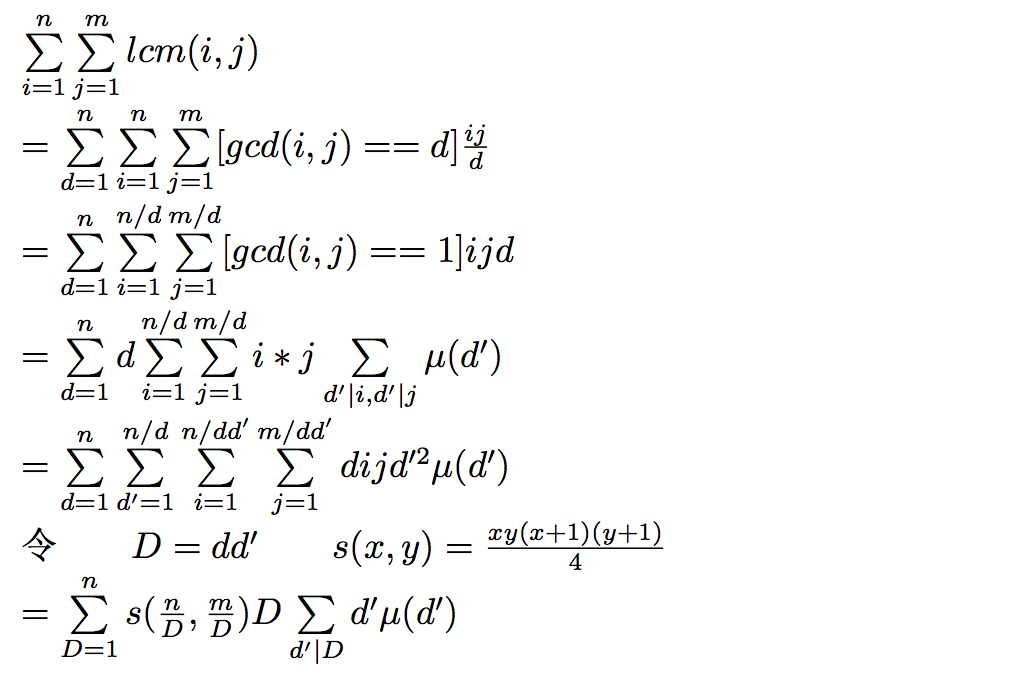
\includegraphics{Mobius.png}
		$$\mu(n) = \begin{cases}
	1 & \text{若}n=1\\
	(-1)^k & \text{若}n\text{无平方数因子,且}n = p_1p_2\dots p_k\\
	0 & \text{若}n\text{有大于}1\text{的平方数因数}
\end{cases}$$
$$\sum_{d|n}{\mu(d)} = \begin{cases}
	1 & \text{若}n=1\\
	0 & \text{其他情况}
\end{cases}$$
$$g(n) = \sum_{d|n}{f(d)} \Leftrightarrow f(n) = \sum_{d|n}{\mu(d)g(\frac{n}{d})}
,       g(x) = \sum_{n=1}^{[x]}f(\frac{x}{n}) \Leftrightarrow f(x) = \sum_{n=1}^{[x]}{\mu(n)g(\frac{x}{n})}$$

		\subsection{Cayley公式与森林计数}
		Cayley公式是说,一个完全图$K_n$有$n^{n-2}$棵生成树,换句话说$n$个节点的带标号的无根树有$n^{n-2}$个。

令$g[i]$表示点数为$i$的森林个数,$f[i]$表示点数为$i$的生成树计数$(f[i]=i^{i-2})$
那么便有$$g[i]=\sum (g[i-j] \times cnr[i-1][j-1] \times f[j])$$
$$g[i]=\sum \frac{g[i-j] \times fac[i-1] \times f[j]}{fac[j-1] \times fac[i-j]}=fac[i-1] \times \sum (\frac{f[j]}{fac[j-1]} \times \frac{g[i-j]}{fac[i-j]})$$
	
	\section{数据结构}
		\subsection{KD Tree}
		\lstinputlisting{KD-tree.cpp}
		\subsection{Splay}
		\lstinputlisting{Splay_xxxxxyt.cpp}
		\subsection{主席树 by xyt}
		\lstinputlisting{主席树_xxxxxyt.cpp}
		\subsection{树链剖分 by cjy}
		\lstinputlisting{树链剖分_cjy.cpp}
		\subsection{树链剖分 by xyt}
		\lstinputlisting{树链剖分_xxxxxyt.cpp}
		\subsection{点分治}
		\lstinputlisting{点分治_xxxxxyt.cpp}
		\subsection{LCT}
		\lstinputlisting{LCT_xxxxxyt.cpp}
	\section{计算几何}
		\subsection{向量旋转}
		\lstinputlisting{向量旋转.cpp}
		\subsection{至少被i个圆覆盖的面积}
		时间复杂度: $n^2logn$
		\lstinputlisting{圆的面积.cpp}
		\subsection{计算几何杂}
		\lstinputlisting{计算几何杂.cpp}
		\subsection{三维变换}
		\lstinputlisting{三维变换.cpp}
	\section{字符串}
		\subsection{Manacher}
		\lstinputlisting{manacher_cjy.cpp}
		\subsection{AC-Automachine by cjy}
		\lstinputlisting{AC-Automachine_cjy.cpp}
		\subsection{AC-Automachine by xyt}
		\lstinputlisting{AC-Automachine_xxxxxyt.cpp}
		\subsection{后缀数组}
		\lstinputlisting{后缀数组_cjy.cpp}
		\subsection{扩展KMP}
		\lstinputlisting{扩展KMP.cpp}
		\subsection{回文树}
		\lstinputlisting{Palindromic_Tree.cpp}
		\subsection{SAM by lss}
		\lstinputlisting{SAM_lss.cpp}
	\section{图论}
		\subsection{图论相关}
		
		1. 差分约束系统\\
  (1)以 x[i] - x[j] <= c 为约束条件,j -> i : c,求最短路得到的是 x[i] <= x[s] 的最大解,存在负权回路无解\\
  (2)以 x[i] - x[j] >= c 为约束条件,j -> i : c,求最长路得到的时 x[i] >= x[s] 的最小解,存在正权回路无解
  // 若有 x[i] = x[j] 则 i <-0-> j\\
2. 最大闭合权子图\\
  s 向正权点连边,负权点向 t 连边,边权为点权绝对值,再按原图连边,边权为INF\\
3. 最大密度子图:max{$\frac{|E'|}{|V'|}$}\\
  (1)猜测答案 g 若最大流大于 EPS 则 g 合法\\
  (2)s -> v: INF, u -> t : INF + g - deg[u], u -> v : 1.00\\
4. 2-SAT\\
  %利用对称性建图,若 u 与 u' 在同一强连通分量中,则无解,若有解输出方案,拓扑排序后自底向上(从 ind = 0 到 otd = 0)选择删除。
  如果Ai与Aj不相容,那么如果选择了Ai,必须选择Aj' ;同样,如果选择了Aj,就必须选择Ai':Ai => Aj',Aj => Ai'(这样的两条边对称)\\
  输出方案:  求图的极大强连通子图 => 缩点并根据原图关系构造一个DAG => 拓扑排 => 自底(被指向的点)向上进行选择删除
(选择当前$id[k][t]$及其后代结点并删除$id[k][t^1]$及其前代结点)\\
5. 最小割\\

(1)二分图最小点权覆盖集:s -> u : w[u], u -> v : INF, v -> t : w[v]\\
  \subsection{斯坦纳树(网格图连接一些确定点的最小生成树)}
$mask:0->2^n$\\
	枚举$mask$的子集更新 $mask':f[i][mask]=max(f[i][mask'] + f[i][mask - mask'])$\\
	最短路更新	$f[j][mask] = f[i][mask] + dis[i][j];$

\subsection{欧拉回路}
判定一个图是否存在欧拉通路或欧拉回路比较容易,这里提供两种不同的判定法则。\\
定理1:一个图有欧拉回路当且仅当它是连通的(即不包括0度的结点)且每个结点都有偶数度。\\
定理2:一个图有欧拉通路当且仅当它是连通的且除两个结点外,其他结点都有偶数度。 \\
定理3:在定理2的条件下,含奇数度的两个结点中,一个必为欧拉通路的起点,另一个必为终点。
\begin{lstlisting}[language=C++]
	void dfs(int x)
	{
    	int y;
   	 	for (int p=hd[x]; p != -1; p=ed[p].next) if (!ed[p].vst) {
       	 	y = ed[p].b;
        	ed[p].vst = 1;
        	ed[p ^ 1].vst = 1;     //如果是有向图则不要这句
        	dfs(y);
        	res[v--] = y + 1;p
    	}
	}
\end{lstlisting}
		\subsection{SteinerTree}
		\lstinputlisting{SteinerTree_cjy.cpp}
		\subsection{LCA}
		\lstinputlisting{LCA_xxxxxyt.cpp}
		\subsection{KM}
		\lstinputlisting{KM.cpp}
		\subsection{KM三次方}
		\lstinputlisting{KM-N^3.cpp}
		\subsection{网络流 by cjy}
		\lstinputlisting{Dinic_cjy.cpp}
		\subsection{网络流 by xyt}
		\lstinputlisting{网络流_xxxxxyt.cpp}
		\subsection{有gap优化的isap}
		\lstinputlisting{有gap优化的isap.cpp}
		\subsection{ZKW费用流}
		\lstinputlisting{ZKW费用流.cpp}
		\subsection{最大密度子图}
		\lstinputlisting{最大密度子图.cpp}
		\subsection{Tarjan}
		\lstinputlisting{tarjan.cpp}
		
		\subsection{K短路}
		\lstinputlisting{k短路.cpp}
		
		\subsection{K短路}
\subsubsection{可重复}
\begin{lstlisting}[language=C++]
#define for_each(it, v) for (vector<Edge*>::iterator it = (v).begin(); it != (v).end(); ++it)
const int MAX_N = 10000, MAX_M = 50000, MAX_K = 10000, INF = 1000000000;
struct Edge {
	int from, to, weight;
};
struct HeapNode {
	Edge* edge;
	int depth;
	HeapNode* child[4];
	//child[0..1] for heap G
	//child[2..3] for heap out edge
};
int n, m, k, s, t, dist[MAX_N];
Edge* edge[MAX_M], prev[MAX_N];
vector<Edge*> graph[MAX_N], graphR[MAX_N];
HeapNode* nullNode, heapTop[MAX_N];
HeapNode* createHeap(HeapNode* curNode, HeapNode* newNode) {
	if (curNode == nullNode) return newNode;
	HeapNode* rootNode = new HeapNode;
	memcpy(rootNode, curNode, sizeof(HeapNode));
	if (newNode->edge->weight < curNode->edge->weight) {
		rootNode->edge = newNode->edge;
		rootNode->child[2] = newNode->child[2];
		rootNode->child[3] = newNode->child[3];
		newNode->edge = curNode->edge;
		newNode->child[2] = curNode->child[2];
		newNode->child[3] = curNode->child[3];
	}
	if (rootNode->child[0]->depth < rootNode->child[1]->depth)
		rootNode->child[0] = createHeap(rootNode->child[0], newNode);
	else
		rootNode->child[1] = createHeap(rootNode->child[1], newNode);
	rootNode->depth=max(rootNode->child[0]->depth, rootNode->child[1]->depth)+1;
	return rootNode;
}
bool heapNodeMoreThan(HeapNode* node1, HeapNode* node2) {
	return node1->edge->weight > node2->edge->weight;
}
int main() {
	scanf("%d%d%d", &n, &m, &k); scanf("%d%d", &s, &t);
	s--, t--;
	while (m--) {
		Edge* newEdge = new Edge;
		int i, j, w; scanf("%d%d%d", &i, &j, &w); i--, j--;
		newEdge->from = i; newEdge->to = j; newEdge->weight = w;
		graph[i].push_back(newEdge); graphR[j].push_back(newEdge);
	}
	//Dijkstra
	queue<int> dfsOrder;
	memset(dist, -1, sizeof(dist));
	typedef pair<int, pair<int, Edge*> > DijkstraQueueItem;
	priority_queue<DijkstraQueueItem, vector<DijkstraQueueItem>, greater<DijkstraQueueItem> > dq;
	dq.push(make_pair(0, make_pair(t, (Edge*) NULL)));
	while (!dq.empty()) {
		int d = dq.top().first, i = dq.top().second.first;
		Edge* edge = dq.top().second.second;
		dq.pop(); if (dist[i] != -1)	continue;
		dist[i] = d; prev[i] = edge;
		dfsOrder.push(i);
		for_each(it, graphR[i]) dq.push(make_pair(d+(*it)->weight, make_pair((*it)->from, *it)));
	}
	//Create edge heap
	nullNode = new HeapNode;
	nullNode->depth = 0;
	nullNode->edge = new Edge;
	nullNode->edge->weight = INF;
	fill(nullNode->child, nullNode->child + 4, nullNode);
	while (!dfsOrder.empty()) {
		int i = dfsOrder.front();  dfsOrder.pop();
		if (prev[i] == NULL) heapTop[i] = nullNode;
		else heapTop[i] = heapTop[prev[i]->to];
		vector<HeapNode*> heapNodeList;
		for_each(it, graph[i])	{
			int j = (*it)->to; if (dist[j] == -1)	continue;
			(*it)->weight += dist[j] - dist[i];
			if (prev[i] != *it) {
				HeapNode* curNode = new HeapNode;
				fill(curNode->child, curNode->child + 4, nullNode);
				curNode->depth = 1; curNode->edge = *it;
				heapNodeList.push_back(curNode);
			}
		}
		if (!heapNodeList.empty()) {   //Create heap out
			make_heap(heapNodeList.begin(), heapNodeList.end(), heapNodeMoreThan);
			int size = heapNodeList.size();
			for (int p = 0; p < size; p++) {
				heapNodeList[p]->child[2] = 2 * p + 1 < size ? heapNodeList[2 * p + 1] : nullNode;
				heapNodeList[p]->child[3] = 2 * p + 2 < size ? heapNodeList[2 * p + 2] : nullNode;
			}
			heapTop[i] = createHeap(heapTop[i], heapNodeList.front());
		}
	}
	//Walk on DAG
	typedef pair<long long, HeapNode*> DAGQueueItem;
	priority_queue<DAGQueueItem, vector<DAGQueueItem>, greater<DAGQueueItem> > aq;
	if (dist[s] == -1) printf("NO\n");
	else {
		printf("%d\n", dist[s]);
		if (heapTop[s] != nullNode)
			aq.push(make_pair(dist[s] + heapTop[s]->edge->weight, heapTop[s]));
	}
	k--;
	while (k--) {
		if (aq.empty()) {printf("NO\n"); continue;}
		long long d = aq.top().first;
		HeapNode* curNode = aq.top().second; aq.pop();
		printf("%I64d\n", d);
		if (heapTop[curNode->edge->to] != nullNode)
			aq.push(make_pair(d + heapTop[curNode->edge->to]->edge->weight, heapTop[curNode->edge->to]));
		for (int i = 0; i < 4; i++)
			if (curNode->child[i] != nullNode)
				aq.push(make_pair(d - curNode->edge->weight + curNode->child[i]->edge->weight, curNode->child[i]));
	}
	return 0;
}
\end{lstlisting}
\subsubsection{不可重复}
\begin{lstlisting}[language=C++]
int Num[10005][205], Path[10005][205], dev[10005];
int from[10005], value[10005], dist[205];
int Next[205], Graph[205][205];
bool forbid[205], hasNext[10005][205];
int N, M, K, s, t, tot, cnt;
struct cmp {
	bool operator() (const int &a, const int &b) {
		int *i, *j;
		if(value[a] != value[b]) return value[a] > value[b];
		for(i = Path[a], j = Path[b]; (*i) == (*j); i ++, j ++);
		return (*i) > (*j);
	}
};
void Check(int idx, int st, int *path, int &res) {
	int i, j;
	for(i = 0; i < N; i ++) {dist[i] = 1000000000; Next[i] = t;}
	dist[t] = 0; forbid[t] = true; j = t;
	while(1) {
		for(i = 0; i < N; i ++)
			if(!forbid[i] && (i != st || !hasNext[idx][j]) && (dist[j] + Graph[i][j] < dist[i] || dist[j] + Graph[i][j] == dist[i] && j < Next[i])) {
				Next[i] = j; dist[i] = dist[j] + Graph[i][j];
			}
		j = -1;
		for(i = 0; i < N; i ++) if(!forbid[i] && (j == -1 || dist[i] < dist[j])) j = i;
		if(j == -1) break; forbid[j] = 1; if(j == st) break;
	}
	res += dist[st];
	for(i = st; i != t; i = Next[i], path ++) (*path) = i;
	(*path) = i;
}
int main() {
	int i, j, k, l;
	while(scanf("%d%d%d%d%d", &N, &M, &K, &s, &t) && N) {
		priority_queue <int, vector <int>, cmp> Q;
		for(i = 0; i < N; i ++)
			for(j = 0; j < N; j ++) Graph[i][j] = 1000000000;
		for(i = 0; i < M; i ++) {
			scanf("%d%d%d", &j, &k, &l); Graph[j - 1][k - 1] = l;
		}
		s --; t --;
		memset(forbid, false, sizeof(forbid));
		memset(hasNext[0], false, sizeof(hasNext[0]));
		Check(0, s, Path[0], value[0]);
		dev[0] = from[0] = Num[0][0] = 0;
		Q.push(0);
		cnt = tot = 1;
		for(i = 0; i < K; i ++) {
			if(Q.empty()) break;
			l = Q.top(); Q.pop();
			for(j = 0; j <= dev[l]; j ++) Num[l][j] = Num[from[l]][j];
			for(; Path[l][j] != t; j ++) {
				memset(hasNext[tot], false, sizeof(hasNext[tot]));
				Num[l][j] = tot ++;
			}
			for(j=0; Path[l][j]!=t;j++) hasNext[Num[l][j]][Path[l][j+1]]=true;
			for(j = dev[l]; Path[l][j] != t; j ++) {
				memset(forbid, false, sizeof(forbid));
				value[cnt] = 0;
				for(k = 0; k < j; k ++) {
					forbid[Path[l][k]] = true; Path[cnt][k] = Path[l][k];
					value[cnt] += Graph[ Path[l][k] ][ Path[l][k + 1] ];
				}
				Check(Num[l][j], Path[l][j], &Path[cnt][j], value[cnt]);
				if(value[cnt] > 2000000) continue;
				dev[cnt] = j; from[cnt] = l;
				Q.push(cnt); cnt ++;
			}
		}
		if(i < K || value[l] > 2000000) printf("None\n");
		else {
			for(i = 0; Path[l][i] != t; i ++) printf("%d-", Path[l][i] + 1);
			printf("%d\n", t + 1);
		}
	}
}
\end{lstlisting}

		
		
		
	\section{其他}
		\subsection{Dancing Links(精确覆盖及重复覆盖)}
		\lstinputlisting{DancingLinksX_xxxxxyt.cpp}
		\subsection{序列莫队}
		\lstinputlisting{序列莫队_xxxxxyt.cpp}
		\subsection{模拟退火}
		\lstinputlisting{模拟退火.cpp}
		\subsection{Java}
		\lstinputlisting{Main.java}

	\section{Tips}
		\lstinputlisting{tips.cpp}
	

	\section{图论}
	\subsection{匈牙利}
	\lstinputlisting{匈牙利.cpp}
	\subsection{hopcroft-karp}
	\lstinputlisting{hopcroft.cpp}
	\subsection{二分图最大权匹配}
	\lstinputlisting{二分图最大权匹配.cpp}
	\subsection{带花树(任意图最大匹配)}
\begin{lstlisting}
//n全局变量,ans是匹配的点数,即匹配数两倍
const int N = 240;
int n, Next[N], f[N], mark[N], visited [N], Link[N], Q[N], head , tail;
vector <int > E[N];
int getf(int x) {return f[x] == x ? x : f[x] = getf(f[x]);}
void merge(int x, int y) {x = getf(x); y = getf(y); if (x != y) f[x] = y;}
int LCA(int x, int y) {
	static int flag = 0;
	flag ++;
	for (; ; swap(x, y)) if (x != -1) {
		x = getf(x);
		if (visited [x] == flag) return x;
		visited [x] = flag;
		if (Link[x] != -1) x = Next[Link[x]];
		else x = -1;
	}
}
void go(int a, int p) {
	while (a != p) {
		int b = Link[a], c = Next[b];
		if (getf(c) != p) Next[c] = b;
		if (mark[b] == 2) mark[Q[tail ++] = b] = 1;
		if (mark[c] == 2) mark[Q[tail ++] = c] = 1;
		merge(a, b); merge (b, c); a = c;
	}
}
void find(int s) {
	for (int i = 0; i < n; i++) {
		Next[i] = -1; f[i] = i;
		mark[i] = 0; visited [i] = -1;
	}
	head = tail = 0; Q[tail ++] = s; mark[s] = 1;
	for (; head < tail && Link[s] == -1; )
		for (int i = 0, x = Q[head ++]; i < (int) E[x]. size (); i++)
			if (Link[x]!=E[x][i]&&getf(x)!=getf(E[x][i])&&mark[E[x][i]]!=2) {
				int y = E[x][i];
				if (mark[y] == 1) {
					int p = LCA(x, y);
					if (getf(x) != p) Next[x] = y;
					if (getf(y) != p) Next[y] = x;
					go(x, p);
					go(y, p);
				} else if (Link[y] == -1) {
					Next[y] = x;
					for (int j = y; j != -1; ) {
						int k = Next[j];
						int tmp = Link[k];
						Link[j] = k;
						Link[k] = j;
						j = tmp;
					}
					break;
				} else {
					Next[y] = x;
					mark[Q[tail ++] = Link[y]] = 1;
					mark[y] = 2;
				}
			}
}
int main () {
	for (int i = 0; i < n; i++) Link[i] = -1;
	for (int i = 0; i < n; i++) if (Link[i] == -1) find(i);
	int ans = 0;
	for (int i = 0; i < n; i++) ans += Link[i] != -1;
}
\end{lstlisting}
	\subsection{仙人掌图判定}
条件是:1.是强连通图;2.每条边在仙人掌图中只属于一个强连通分量。//
仙人掌图的三个性质:1.仙人掌dfs图中不能有横向边,简单的理解为每个点只能出现在一个强联通分量中;//
2.low[v]<dfn[u],其中u为v的父节点;//
3.a[u]+b[u]<2,a[u]为u节点的儿子节点中有a[u]个low值小于u的dfn值,b[u]为u的逆向边条数。//
\begin{lstlisting}[language=C++]
bool tarjan(int x) {
	dfn[x] = low[x] = ++cnt;
	stack[++top] = x; ins[x] = 1;
	int num = 0;
	for (int now = g[x]; now; now = pre[now]) {
		int y = nex[now];
		if (!dfn[y]) {
			if (!tarjan(y)) return 0;
			if (low[y] > dfn[x]) return 0;
			if (low[y] < dfn[x]) num++;
			low[x] = min(low[x], low[y]);
		} else if (ins[y]) {
			num++;
			low[x] = min(low[x], dfn[y]);
		} else return 0;
	}
	if (num >= 2) return 0;
	if (low[x] == dfn[x]) {
		while (stack[top] != x) {
			int y = stack[top];
			ins[y] = 0;
			stack[top--] = 0;
		}
		ins[x] = 0;
		stack[top--] = 0;
	}
	return 1;
}
\end{lstlisting}
	
	\subsection{最小树形图}
	\subsection{无向图最小割}
\begin{lstlisting}
//0base,g是图的邻接矩阵,复杂度O(n^3)
#define typec int // type of res注意具体范围
const typec inf = 0x3f3f3f3f; // max of res
const typec maxw = 1000; // maximum edge weight
typec g[V][V], w[V] ;
int a[V], v[V], na[V];
typec mincut(int n){
	int i, j, pv, zj;
	typec best = maxw * n * n;
	for (i = 0; i < n; i++) v[i] = i;
	while (n > 1) {
		for (a[v[0]] = 1, i = 1; i < n; i++) {
			a[v[i]] = 0; na[i - 1] = i;
			w[i] = g[v[0]][v[i]];
		}
		for (pv = v[0], i = 1; i < n; i++ ) {
			for (zj = -1, j = 1; j < n; j++ )
				if (!a[v[j]] && (zj < 0 || w[j] > w[zj])) zj = j;
			a[v[zj]] = 1;
			if (i == n - 1) {
				if (best > w[zj]) best = w[zj];
				for (i=0; i<n; i++) g[v[i]][pv]=g[pv][v[i]]+=g[v[zj]][v[i]];
				v[zj] = v[--n];
				break;
			}
			pv = v[zj];
			for (j = 1; j < n; j++) if(!a[v[j]]) w[j] += g[v[zj]][v[j]];
		}
	}
	return best;
}
\end{lstlisting}
	\lstinputlisting{最小树形图.cpp}
	\subsection{zkw费用流}
	使用条件:费用非负
	%\lstinputlisting{zkw.cpp}
	\subsection{上下界网络流}
原图中边流量限制为(a,b),增加一个新的源点S’,汇点T’,对于每个顶点,\\
向S’连容量为所有流入它的边的下界和的边,向T’连容量为所有它流出的下界和的边,\\
T’向S’连容量为无穷大的边,第一次跑S’ 到T’ 的网络流,判断S’流出的边是否满流,\\
即可判断是否有可行解,然后再跑S 到T的网络流,总流量为两次之和。

$B(u,v)$表示边$(u,v)$流量的下界,$C(u,v)$表示边$(u,v)$流量的上界,$F(u,v)$表示边$(u,v)$的流量。设$G(u,v) = F(u,v) - B(u,v)$,显然有
	$$0 \leq G(u,v) \leq C(u,v)-B(u,v)$$

\subsubsection{无源汇的上下界可行流}

建立超级源点$S^*$和超级汇点$T^*$,对于原图每条边$(u,v)$在新网络中连如下三条边:$S^* \rightarrow v$,容量为$B(u,v)$;$u \rightarrow T^*$,容量为$B(u,v)$;$u \rightarrow v$,容量为$C(u,v) - B(u,v)$。最后求新网络的最大流,判断从超级源点$S^*$出发的边是否都满流即可,边$(u,v)$的最终解中的实际流量为$G(u,v)+B(u,v)$。

\subsubsection{有源汇的上下界可行流}

从汇点$T$到源点$S$连一条上界为$\infty$,下界为$0$的边。按照\textbf{无源汇的上下界可行流}一样做即可,流量即为$T \rightarrow S$边上的流量。

\subsubsection{有源汇的上下界最大流}

\begin{enumerate}
	\item 在\textbf{有源汇的上下界可行流}中,从汇点$T$到源点$S$的边改为连一条上界为$\infty$,下届为$x$的边。$x$满足二分性质,找到最大的$x$使得新网络存在\textbf{无源汇的上下界可行流}即为原图的最大流。
	\item 从汇点$T$到源点$S$连一条上界为$\infty$,下界为$0$的边,变成无源汇的网络。按照\textbf{无源汇的上下界可行流}的方法,建立超级源点$S^*$和超级汇点$T^*$,求一遍$S^* \rightarrow T^*$的最大流,再将从汇点$T$到源点$S$的这条边拆掉,求一次$S \rightarrow T$的最大流即可。
\end{enumerate}

\subsubsection{有源汇的上下界最小流}

\begin{enumerate}
	\item 在\textbf{有源汇的上下界可行流}中,从汇点$T$到源点$S$的边改为连一条上界为$x$,下界为$0$的边。$x$满足二分性质,找到最小的$x$使得新网络存在\textbf{无源汇的上下界可行流}即为原图的最小流。
	\item 按照\textbf{无源汇的上下界可行流}的方法,建立超级源点$S^*$与超级汇点$T^*$,求一遍$S^* \rightarrow T^*$的最大流,但是注意这一次不加上汇点$T$到源点$S$的这条边,即不使之改为无源汇的网络去求解。求完后,再加上那条汇点$T$到源点$S$上界$\infty$的边。因为这条边下界为$0$,所以$S^*$,$T^*$无影响,再直接求一次$S^* \rightarrow T^*$的最大流。若超级源点$S^*$出发的边全部满流,则$T \rightarrow S$边上的流量即为原图的最小流,否则无解。
\end{enumerate}



	\subsection{一般图最大匹配}
	\lstinputlisting{一般图最大匹配.cpp}
	\subsection{无向图全局最小割}
	注意事项:处理重边时,应该对边权累加
	\lstinputlisting{无向图全局最小割.cpp}
	\subsection{有根树的同构}
	\lstinputlisting{有根树的同构.cpp}
	\subsection{弦图性质}
\begin{itemize}
  % \item 团数 $\le$ 色数
  % \item 最大独立集数 $\le$ 最小团覆盖数
\item 任何一个弦图都至少有一个单纯点, 不是完全图的弦图至少有两个不相邻的单纯点.
\item 设第i个点在弦图的完美消除序列第 $p(i)$个. 令 $N(v) = \{w | w \text{与} v \text{相邻且} p(w) > p(v) \}$弦图的极大团一定是 $v \cup N(v)$ 的形式.
\item 弦图最多有$n$个极大团.
\item 设 $next(v)$ 表示 $N(v)$中最前的点. 令 $w*$ 表示所有满足 $A\in B$ 的 $w$ 中最后的一个点.
  判断 $v \cup N(v)$是否为极大团,
  只需判断是否存在一个 $w$,
  满足 $Next(w) = v$ 且 $|N(v)| + 1 \le |N(w)|$ 即可.
\item 最小染色:完美消除序列从后往前依次给每个点染色, 给每个点染上可以染的最小的颜色. (团数 = 色数)
\item 最大独立集:完美消除序列从前往后能选就选.
\item 最小团覆盖:设最大独立集为 $\{p_1, p_2, \ldots, p_t\}$, 则 $\{p_1 \cup N(p_1), \ldots, p_t \cup N(p_t) \}$为最小团覆盖.  (最大独立集数 = 最小团覆盖数)
\end{itemize}
\subsection{弦图判定}
\lstinputlisting{弦图的判定.cpp}
\subsection{弦图求团数}
\lstinputlisting{弦图求团数.cpp}
\subsection{哈密尔顿回路(ORE性质的图)}
ORE性质:$\forall x,y \in V \wedge (x,y) \notin E \ \ s.t. \ \ deg_x+deg_y \geq n$返回结果:从顶点$1$出发的一个哈密尔顿回路.使用条件:$n \geq 3$
\lstinputlisting{哈密尔顿.cpp}
\subsection{度限制生成树}
\lstinputlisting{度限制生成树.cpp}


	\section{数值}
	\subsection{行列式取模}
	\lstinputlisting{detmod.cpp}
	\subsection{最小二乘法}
	\lstinputlisting{最小二乘法.cpp}
	\subsection{多项式求根}
	\lstinputlisting{多项式求根.cpp}
	\subsection{单纯形}
	返回结果:$max\{c_{1 \times m} \cdot x_{m \times 1} \ | \ x_{m \times 1} \geq 0_{m \times 1}, a_{n \times m} \cdot x_{m \times 1} \leq b_{n \times 1}\}$

	\lstinputlisting{单纯形.cpp}
	\subsection{辛普森}
	\lstinputlisting{辛普森.cpp}
	\subsection{线性规划}
\begin{lstlisting}[language=C++]
//N[0]代表N中的元素个数,B[0]代表B中的元素个数。
//读入格式:首先两个数n, m,表示未知数的数量和约束的数量。接下来一行n个数,为目标函数的系数。然后m行,每行m+1个数,表示一个约束。前m个数是系数,最后一个是常数项。
//输出格式:如果无解,只有一行"Infeasible"。如果解可以无穷大,只有一行"Unbounded"。否则,第一行为最大的目标函数值,接下来是每个未知数的值。
const double eps = 1e-10;
const int MAXSIZE = 2000, oo = 19890709;
double v, A[MAXSIZE+1][MAXSIZE+1], tA[MAXSIZE+1][MAXSIZE+1];
double b[MAXSIZE+1], tb[MAXSIZE+1], c[MAXSIZE+1], tc[MAXSIZE+1];
int n, m, N[MAXSIZE+1+1], B[MAXSIZE+1+1];
class LinearProgramming {
	void read() {
		scanf("%d%d", &n, &m);
		for(int i=1; i<=n; i++) scanf("%lf", &c[i]);
		for(int i=1; i<=m; i++) {
			for(int j=1; j<=n; j++) scanf("%lf", &A[n+i][j]);
			scanf("%lf", &b[n+i]);
		}
	}
	void pivot(int l, int e) {
		tb[e] = b[l]/A[l][e]; tA[e][l] = 1/A[l][e];
		for(int i=1; i<=N[0]; i++) if (N[i] != e) tA[e][N[i]] = A[l][N[i]]/A[l][e];
		for(int i=1; i<=B[0]; i++) {
			tb[B[i]] = b[B[i]]-A[B[i]][e]*tb[e]; tA[B[i]][l] = -A[B[i]][e]*tA[e][l];
			for(int j=1; j<=N[0]; j++)
				if (N[j] != e) tA[B[i]][N[j]] = A[B[i]][N[j]]-tA[e][N[j]]*A[B[i]][e];
		}
		v += tb[e]*c[e]; tc[l] = -tA[e][l]*c[e];
		for(int i=1; i<=N[0]; i++) if (N[i] != e) tc[N[i]] = c[N[i]]-tA[e][N[i]]*c[e];
		for(int i=1; i<=N[0]; i++) if (N[i] == e) N[i] = l;
		for(int i=1; i<=B[0]; i++) if (B[i] == l) B[i] = e;
		for(int i=1; i<=B[0]; i++) {
			for(int j=1; j<=N[0]; j++) A[B[i]][N[j]] = tA[B[i]][N[j]];
			b[B[i]] = tb[B[i]];
		}
		for(int i=1; i<=N[0]; i++) c[N[i]] = tc[N[i]];
	}
	bool opt() { //false stands for unbounded
		while (true) {
			int l, e; double maxUp = -1;//不能是0!
			for(int ie=1; ie<=N[0]; ie++) {
				int te = N[ie]; if (c[te] <= eps) continue;  //eps or 0
				double delta = oo; int tl = MAXSIZE+1;
				for(int i=1; i<=B[0]; i++)
					if (A[B[i]][te] > eps) {  //eps or 0
						double temp = b[B[i]]/A[B[i]][te];
						if (delta == oo || temp < delta || temp == delta && B[i] < tl) {
							delta = temp; tl = B[i];
						}
					}
				if (tl == MAXSIZE+1) return false;
				if (delta*c[te] > maxUp) {
					maxUp = delta*c[te]; l = tl; e = te;
				}
			}
			if (maxUp == -1) break; pivot(l, e);
		}
		return true;
	}
	void delete0() {
		int p;
		for(p=1; p<=B[0]; p++) if (B[p] == 0) break;
		if (p <= B[0]) pivot(0, N[1]);
		for(p=1; p<=N[0]; p++) if (N[p] == 0) break;
		for(int i=p; i<N[0]; i++) N[i] = N[i+1];
		N[0]--;
	}
	bool initialize() {
		N[0] = B[0] = 0;
		for(int i=1; i<=n; i++) N[++N[0]] = i;
		for(int i=1; i<=m; i++) B[++B[0]] = n+i;
		v = 0; int l = B[1];
		for(int i=2; i<=B[0]; i++) if (b[B[i]] < b[l]) l = B[i];
		if (b[l] >= 0) return true;
		double origC[MAXSIZE+1];
		memcpy(origC, c, sizeof(double)*(n+m+1));
		N[++N[0]] = 0;
		for(int i=1; i<=B[0]; i++) A[B[i]][0] = -1;
		memset(c, 0, sizeof(double)*(n+m+1));
		c[0] = -1; pivot(l, 0);
		opt();//unbounded????
		if (v < -eps) return false;//eps
		delete0();
		memcpy(c, origC, sizeof(double)*(n+m+1));
		bool inB[MAXSIZE+1];
		memset(inB, false, sizeof(bool)*(n+m+1));
		for(int i=1; i<=B[0]; i++) inB[B[i]] = true;
		for(int i=1; i<=n+m; i++)
			if (inB[i] && c[i] != 0) {
				v += c[i]*b[i];
				for(int j=1; j<=N[0]; j++) c[N[j]] -= A[i][N[j]]*c[i];
				c[i] = 0;
			}
		return true;
	}
	public: void simplex(string inputName, string outputName) {
		freopen(inputName.c_str(), "r", stdin);
		freopen(outputName.c_str(), "w", stdout);
		read();
		if (!initialize()) {
			printf("Infeasible\n");
			return;
		}
		if (!opt()) {
			printf("Unbounded\n");
			return
		} else printf("Max value is %lf\n", v);
		bool inN[MAXSIZE+1];
		memset(inN, false, sizeof(bool)*(n+m+1));
		for(int i=1; i<=N[0]; i++) inN[N[i]] = true;
		for(int i=1; i<=n; i++)
			if (inN[i]) printf("x%d = %lf\n", i, 0.0);
			else printf("x%d = %lf\n", i, b[i]);
	}
};
int main() {
	LinearProgramming test;
	test.simplex("a.in", "a.out");
}
\end{lstlisting}
	
	
	
	\section{数论}
	\subsection{离散对数}
	\lstinputlisting{离散对数.cpp}
	\subsection{原根}
	$x$为$p$的原根当且仅当对$p-1$任意质因子$k$有$x^{k}\neq 1(\text{mod } p)$.
	\subsection{Miller Rabin and Rho}
	\lstinputlisting{Miller.cpp}
	\subsection{exgcd}
	\lstinputlisting{exgcd.cpp}
	\subsection{离散平方根}
	\lstinputlisting{离散平方根.cpp}
	\subsection{$O(m^2 \log(n))$求线性递推}
	已知$a_0, a_1, ..., a_{m - 1}$$a_n = c_0 * a_{n - m} + ... + c_{m - 1} * a_{n - 1}$求$a_n = v_0 * a_0 + v_1 * a_1 + ... + v_{m - 1} * a_{m - 1}$
	\lstinputlisting{线性递推.cpp}
	\subsection{CRT}
	\lstinputlisting{CRT.cpp}
	\subsection{佩尔方程求根$x^2-n*y^2=1$}
	\lstinputlisting{pell.cpp}
	\subsection{直线下整点个数}
	求$\displaystyle\sum_{i=0}^{n-1} \lfloor\frac{a+bi}{m}\rfloor$.
	\lstinputlisting{直线下整点个数.cpp}
	
	
	\section{字符串}
	\subsection{ex-KMP}
	返回结果:$next_i = lcp(text, text_{i \dots n-1})$
	\lstinputlisting{exkmp.cpp}
	\subsection{串最小表示}
	\lstinputlisting{串最小表示.cpp}
	
	\section{其他}
	\subsection{某年某月某日是星期几}
	\lstinputlisting{date.cpp}
	\subsection{枚举k子集}
	\lstinputlisting{ksub.cpp}
	\subsection{环状最长公共子串}
	\lstinputlisting{环状最长公共子串.cpp}
	\subsection{LL*LLmodLL}
	\lstinputlisting{LLmod.cpp}
	\subsection{曼哈顿最小生成树}
	\lstinputlisting{曼哈顿最小生成树.cpp}
	\subsection{极大团计数}
	\lstinputlisting{极大团计数.cpp}
	\subsection{最大团搜索}
	Int g[][]为图的邻接矩阵.MC(V)表示点集V的最大团.令Si={vi, vi+1, ..., vn}, mc[i]表示MC(Si).倒着算mc[i],那么显然MC(V)=mc[1].此外有mc[i]=mc[i+1] or mc[i]=mc[i+1]+1.
	\lstinputlisting{最大团搜索.cpp}
	\subsection{DLX精确覆盖}
	\lstinputlisting{DLX.cpp}
	\subsection{DLX重复覆盖}
	\lstinputlisting{DLX_multi.cpp}
	\subsection{Java}
	\lstinputlisting[language = java]{template.java}
	\subsection{Java分数类}
	\lstinputlisting[language = java]{fraction.java}
	\subsection{Java Big}
	\lstinputlisting[language = java]{biginteger.java}
\subsection{关同步}
\begin{lstlisting}[language=C++]
    std::ios::sync_with_stdio(false);
\end{lstlisting}
	\subsection{crope}
	\begin{lstlisting}
#include <ext/rope>
using __gnu_cxx::crope; using __gnu_cxx::rope;
a = b.substr(from, len); // [from, from + len)
a = b.substr(from);      // [from, from]
b.c_str();               // might lead to memory leaks
b.delete_c_str();        // delete the c_str that created before
a.insert(p, str);        // insert str before position p
a.erase(i, n);           // erase [i, i + n)

	\end{lstlisting}	
	\end{multicols}

	\begin{multicols}{2}%\tiny
	\section{Hints}

	\subsection{线性规划对偶}
	maximize $\bm{c}^T\bm{x}$, subject to $\bm{Ax} \leq \bm{b}$, $\bm{x} \geq 0$.\\
	minimize $\bm{y}^T\bm{b}$, subject to $\bm{y}^T\bm{A} \geq \bm{c}^T$ , $\bm{y} \geq 0$.
	\subsection{博弈论相关}
\begin{enumerate}
	\item Anti-SG:
		规则与Nim基本相同,取最后一个的输。
		先手必胜当且仅当:
		(1) 所有堆的石子数都为1且游戏的SG值为0;
		(2) 有些堆的石子数大于1且游戏的SG值不为0。
	\item SJ定理:
		对于任意一个Anti-SG游戏,如果我们规定当局面中,所有的单一游戏的SG值为0 时,游戏结束,则先手必胜当且仅当:
		(1) 游戏的SG函数不为0且游戏中某个单一游戏的SG函数大于1;
		(2) 游戏的SG函数为0且游戏中没有单一游戏的SG函数大于1。
	\item Multi-SG游戏:
		可以将一堆石子分成多堆.
	\item Every-SG游戏:
		每一个可以移动的棋子都要移动.
		对于我们可以赢的单一游戏,我们一定要拿到这一场游戏的胜利.
		只需要考虑如何让我们必胜的游戏尽可能长的玩下去,对手相反。
		于是就来一个DP,
		step[v] = 0;(v为终止状态)
		step[v] = max{step[u]} + 1;(sg[v]>0,sg[u]=0)
		step[v] = min{step[u]} + 1;(sg[v]==0)
	\item 翻硬币游戏:
		N枚硬币排成一排,有的正面朝上,有的反面朝上。游戏者根据某些约束翻硬币(如:每次只能翻一或两枚,或者每 次只能翻连续的几枚),但他所翻动的硬币中,最右边的必须是从正面翻到反面。谁不能翻谁输。
		结论:局面的SG值为局面中每个正面朝上的棋子单一存在时的SG值的异或和。可用数学归纳法证明。
	\item 无向树删边游戏:
		规则如下:
		给出一个有N个点的树,有一个点作为树的根节点。游戏者轮流从树中删去边,删去一条边后,不与根节点相连的部分将被移走。谁无路可走谁输。
		结论:
		叶子节点的SG值为0;中间节点的SG值为它的所有子节点的SG值加1后的异或和。是用数学归纳法证明。
	\item Christmas Game(PKU3710):
		题目大意:
		有N个局部联通的图。Harry和Sally轮流从图中删边,删去一条边后,不与根节点相连的部分将被移走。Sally为先手。图是通过从基础树中加一些边得到的。所有形成的环保证不共用边,且只与基础树有一个公共点。谁无路可走谁输。环的处理成为了解题的关键。
		性质:
		(1)对于长度为奇数的环,去掉其中任意一个边之后,剩下的两个链长度同奇偶,抑或之后的SG值不可能为奇数,所以它的SG值为1;\\
		(2)对于长度为偶数的环,去掉其中任意一个边之后,剩下的两个链长度异奇偶,抑或之后的SG值不可能为0,所以它的SG值为0;所以我们可以去掉所有的偶环,将所有的奇环变为长短为1 的链。
		这样的话,我们已经将这道题改造成了上一节的模型。
	\item 无向图的删边游戏:
		我们将Christmas Game这道题进行一步拓展——去掉对环的限制条件,这个模型应该怎样处理?
		无向图的删边游戏:
		一个无向联通图,有一个点作为图的根。游戏者轮流从图中删去边,删去一条边后,不与根节点相连的部 分将被移走。谁无路可走谁输。
		结论:
		对无向图做如下改动:将图中的任意一个偶环缩成一个新点,任意一个奇环缩成一个新点加一个新边;所有连到原先环上的边全部改为与新点相连。这样的改动不会影响图的SG值。
	\item Staircase nim:
		楼梯从地面由下向上编号为0到n。游戏者在每次操作时可以将楼梯j(1<=j<=n)上的任意多但至少一个硬币移动到楼梯j-1 上。将最后一枚硬币移至地上的人获胜。
		结论:
		设该游戏Sg函数为奇数格棋子数的Xor和S。
		如果S=0,则先手必败,否则必胜。
\end{enumerate}




\subsection{无向图最小生成树计数}
kirchhoff矩阵 = 度数矩阵($i = j$, $d[i][j]$ = 度数) - 邻接矩阵(i、j之间有边, $a[i][j] = 1$)\\
不同的生成树个数等于任意n - 1主子式行列式的绝对值

\subsection{最小覆盖构造解}
从X中所有的未盖点出发扩展匈牙利树,标记树中的所有点,则X中的未标记点和Y中的已标记点组成了所求的最小覆盖。

\subsection{常用数学公式}
\subsubsection{斐波那契数列}

\begin{enumerate}
	\item $fib_0=0, fib_1=1, fib_n=fib_{n-1}+fib_{n-2}$
	\item $fib_{n+2} \cdot fib_n-fib_{n+1}^2=(-1)^{n+1}$
	\item $fib_{-n}=(-1)^{n-1}fib_n$
	\item $fib_{n+k}=fib_k \cdot fib_{n+1}+fib_{k-1} \cdot fib_n$
	\item $gcd(fib_m, fib_n)=fib_{gcd(m, n)}$
	\item $fib_m|fib_n^2\Leftrightarrow nfib_n|m$
\end{enumerate}

\subsubsection{错排公式}

\begin{enumerate}
	\item $D_n = (n-1)(D_{n-2}-D_{n-1})
	= n! \cdot (1-\frac{1}{1!}+\frac{1}{2!}-\frac{1}{3!}+\ldots+\frac{(-1)^n}{n!})$
\end{enumerate}

\subsubsection{莫比乌斯函数}

$$\mu(n) = \begin{cases}
	1 & \text{若}n=1\\
	(-1)^k & \text{若}n\text{无平方数因子,且}n = p_1p_2\dots p_k\\
	0 & \text{若}n\text{有大于}1\text{的平方数因数}
\end{cases}$$
$$\sum_{d|n}{\mu(d)} = \begin{cases}
	1 & \text{若}n=1\\
	0 & \text{其他情况}
\end{cases}$$
$$g(n) = \sum_{d|n}{f(d)} \Leftrightarrow f(n) = \sum_{d|n}{\mu(d)g(\frac{n}{d})}
,       g(x) = \sum_{n=1}^{[x]}f(\frac{x}{n}) \Leftrightarrow f(x) = \sum_{n=1}^{[x]}{\mu(n)g(\frac{x}{n})}$$

\subsubsection{五边形数定理}

设$p(n)$是$n$的拆分数,有$p(n) = \sum_{k \in \mathbb{Z} \setminus \{0\}} (-1)^{k - 1} p\left(n - \frac{k(3k - 1)}{2}\right)$

\subsubsection{树的计数}

\begin{enumerate}
	\item 有根树计数:$n+1$个结点的有根树的个数为
		$a_{n+1} = \frac{\sum_{j=1}^{n}{j \cdot a_j \cdot{S_{n, j}}}}{n}$
	其中,
		$S_{n, j} = \sum_{i=1}^{n/j}{a_{n+1-ij}} = S_{n-j, j} + a_{n+1-j}$
	\item 无根树计数:当$n$为奇数时,$n$个结点的无根树的个数为
		$a_n-\sum_{i=1}^{n/2}{a_ia_{n-i}}$
	当$n$为偶数时,$n$个结点的无根树的个数为
		$a_n-\sum_{i=1}^{n/2}{a_ia_{n-i}}+\frac{1}{2}a_{\frac{n}{2}}(a_{\frac{n}{2}}+1)$
	\item $n$个结点的完全图的生成树个数为
		$n^{n-2}$
	\item 矩阵-树定理:图$G$由$n$个结点构成,设$\bm{A}[G]$为图$G$的邻接矩阵、$\bm{D}[G]$为图$G$的度数矩阵,则图$G$的不同生成树的个数为$\bm{C}[G] = \bm{D}[G] - \bm{A}[G]$的任意一个$n-1$阶主子式的行列式值。
\end{enumerate}

\subsubsection{欧拉公式}

平面图的顶点个数、边数和面的个数有如下关系:
	$V - E + F = C+ 1$
\indent 其中,$V$是顶点的数目,$E$是边的数目,$F$是面的数目,$C$是组成图形的连通部分的数目。
$V - E + F = 2 - 2G$
\indent 其中,$G$ is the number of genus of surface

\subsubsection{皮克定理}

给定顶点坐标均是整点(或正方形格点)的简单多边形,其面积$A$ 和内部格点数目$i$、边上格点数目$b$的关系:
	$$A = i + \frac{b}{2} - 1$$


\subsection{平面几何公式}
\subsubsection{三角形和四边形的费马点}
  \begin{itemize}
  \item 费马点: 距几个顶点距离之和最小的点
  \item 三角形:
      若每个角都小于 $120^{\circ}$: 以每条边向外作正三角形, 得到 $\Delta ABF$, $\Delta BCD$, $\Delta CAE$, 连接$AD$, $BE$, $CF$, 三线必共点于费马点. 该点对三边的张角必然是$120^{\circ}$, 也必然是三个三角形外接圆的交点。否则费马点一定是那个大于等于$120^{\circ}$的顶角
  \item 四边形:
        在凸四边形中, 费马点为对角线的交点,在凹四边形中, 费马点位凹顶点
\end{itemize}
\subsubsection{四边形}

$D_1, D_2$为对角线,$M$对角线中点连线,$A$为对角线夹角,$p$ 为半周长
\begin{enumerate}
	\item $a^2+b^2+c^2+d^2=D_1^2+D_2^2+4M^2$
	\item $S=\frac{1}{2}D_1D_2sinA$
	\item 对于圆内接四边形
		$ac+bd=D_1D_2$
	\item 对于圆内接四边形
		$S=\sqrt{(p-a)(p-b)(p-c)(p-d)}$
\end{enumerate}

\subsubsection{棱台}

\begin{enumerate}
	\item 体积
		$V=(A_1+A_2+\sqrt{A_1A_2}) \cdot \frac{h}{3}$
		$A_1,A_2$为上下底面积,$h$为高
\end{enumerate}

\subsubsection{圆台}

\begin{enumerate}
	\item 母线
		$l=\sqrt{h^2+(r_1-r_2)^2}$
	,  侧面积
		$S=\pi(r_1+r_2)l$
	,  全面积
		$T=\pi r_1(l+r_1)+\pi r_2(l+r_2)$
	,  体积
		$V=\frac{\pi}{3}(r_1^2+r_2^2+r_1r_2)h$
\end{enumerate}

\subsubsection{球台}

\begin{enumerate}
	\item 侧面积
		$S=2\pi rh$
	,    全面积
		$T=\pi(2rh+r_1^2+r_2^2)$
	,    体积
		$V=\frac{\pi h[3(r_1^2+r_2^2)+h^2]}{6}$
\end{enumerate}

\subsubsection{球扇形}

\begin{enumerate}
	\item 全面积
		$T=\pi r(2h+r_0)$
		$h$为球冠高,$r_0$为球冠底面半径
	,   体积
		$V=\frac{2}{3}\pi r^2h$
\end{enumerate}

\subsection{立体几何公式}

\subsubsection{球面三角公式}

设$a, b, c$是边长,$A, B, C$是所对的二面角,
有余弦定理$cos a = cos b \cdot cos c + sin b \cdot sin c \cdot cos A$
正弦定理$\frac{sin A}{sin a} = \frac{sin B}{sin b} = \frac{sin C}{sin c}$
三角形面积是$A + B + C - \pi$

\subsubsection{四面体体积公式}

$U, V, W, u, v, w$是四面体的$6$条棱,$U, V, W$构成三角形,$(U, u), (V, v), (W, w)$ 互为对棱,
则$$V = \frac{\sqrt{(s - 2a)(s - 2b)(s - 2c)(s - 2d)}}{192 uvw}$$
其中$
        a  =  \sqrt{xYZ},
        b  =  \sqrt{yZX},
        c  =  \sqrt{zXY},
        d  =  \sqrt{xyz},
        s  =  a + b + c + d
    $

\subsubsection{三次方程求根公式}
对一元三次方程
$x ^ 3 + px + q = 0$,
令
\begin{align*}
  A = \sqrt[3]{-\frac{q}{2}+\sqrt{(\frac{q}{2})^2+(\frac{p}{3})^3}},
  B = \sqrt[3]{-\frac{q}{2}-\sqrt{(\frac{q}{2})^2+(\frac{p}{3})^3}},
  \omega = \frac{(-1 + \mathrm{i} \sqrt{3})}{2}
\end{align*}

则 $x_j = A\omega^{j} + B\omega^{2j}$ (j = 0, 1, 2).

当求解 $ax ^ 3 + bx ^ 2 + cx + d = 0$ 时, 令$x = y - \frac{b}{3a}$, 再求解$y$, 即转化为$y^3 + py + q = 0$ 的形式.
其中,
\begin{align*}
  p = \frac{b^2 - 3ac}{3a^2},
  q = \frac{2b ^ 3 - 9 abc + 27 a ^ 2 d}{27 a ^ 3}
\end{align*}

卡尔丹判别法:
令$\Delta = (\frac{q}{2}) ^ 2 + (\frac{p}{3}) ^ 3$.
当$\Delta > 0$时, 有一个实根和一对个共轭虚根;
当$\Delta = 0$时, 有三个实根, 其中两个相等;
当$\Delta < 0$时, 有三个不相等的实根.

\subsubsection{椭圆}
\begin{itemize}
\item 椭圆$\frac{x^2}{a^2} + \frac{y^2}{b^2} = 1$, 其中离心率$e = \frac{c}{a}, c = \sqrt{a^2 - b^2}$; 焦点参数$p = \frac{b^2}{a}$
\item 椭圆上$(x, y)$点处的曲率半径为$R = a^2 b^2 (\dfrac{x^2}{a^4} + \dfrac{y^2}{b^4})^\frac{3}{2} = \dfrac{(r_1 r_2)^\frac{3}{2}}{ab}$, 其中$r_1$ 和$r_2$ 分别为$(x, y)$与两焦点$F_1$和$F_2$的距离. %设点$A$和点$M$的坐标分别为$(a, 0)$ 和$(x, y)$, 则$AM$的弧长为
  \[ L_{AM} = a \int_0^{\arccos{\frac{x}{a} }} \sqrt{1 - e^2 \cos^2 t} \textrm{d} t = a \int_{\arccos{\frac{x}{a} }}^\frac{\pi}{2} \sqrt{1 - e^2 \sin^2 t} \textrm{d} t\]
\item 椭圆的周长$L = 4a \int_0^{\frac{\pi}{2}} \sqrt{1 - e^2 \sin^2 t } \textrm{d} t = 4a E(e, \frac{\pi}{2})$, 其中
  \[ E(e, \frac{\pi}{2}) = \frac{\pi}{2} [ 1 - (\frac{1}{2})^2 e^2 - (\frac{1 \times 3}{2 \times 4})^2 \frac{e^4}{3} - (\frac{1 \times 3 \times 5}{2 \times 4 \times 6})^2 \frac{e^6}{5} - \cdots\]
\item 设椭圆上点$M(x, y), N(x, -y), x, y > 0, A(a, 0)$, 原点$O(0, 0)$, 扇形$OAM$ 的面积$S_{OAM} = \frac{1}{2} ab \arccos{\frac{x}{a}}$, 弓形$MAN$的面积$S_{MAN} = ab \arccos{\frac{x}{a}} - xy$.
\item 需要$5$个点才能确定一个圆锥曲线.
\item 设$\theta$为$(x, y)$点关于椭圆中心的极角, $r$为$(x, y)$到椭圆中心的距离, 椭圆极坐标方程:
  \[ x = r \cos \theta, y = r \sin \theta, r^2 = \frac{b^2 a^2}{b^2 \cos^2 \theta + a^2 \sin^2 \theta}\]
\end{itemize}

\subsubsection{抛物线}
\begin{itemize}
\item 标准方程$y^2 = 2px$, 曲率半径$ R = \dfrac{(p + 2x)^{\frac{3}{2} }}{\sqrt{p}}$
\item 弧长: 设$M(x, y)$是抛物线上一点, 则$L_{OM} = \frac{p}{2} [ \sqrt{\frac{2x}{p}(1 + \frac{2x}{p})} + \ln(\sqrt{\frac{2x}{p}} + \sqrt{1 + \frac{2x}{p}})]$
\item 弓形面积: 设$M, D$是抛物线上两点, 且分居一, 四象限. 做一条平行于$MD$且与抛物线相切的直线$L$. 若$M$到$L$的距离为$h$. 则有$S_{MOD} = \frac{2}{3}MD \cdot h$.
\end{itemize}

\subsubsection{重心}
\begin{itemize}
\item 半径$r$, 圆心角为$\theta$的扇形的重心与圆心的距离为$\dfrac{4r\sin\frac{\theta}{2}}{3\theta}$
\item 半径$r$, 圆心角为$\theta$的圆弧的重心与圆心的距离为$\dfrac{4r\sin^3\frac{\theta}{2}}{3(\theta - \sin\theta)}$
\item 椭圆上半部分的重心与圆心的距离为$\dfrac{4b}{3\pi}$
\item  抛物线中弓形$MOD$的重心满足$CQ = \frac{2}{5} PQ$, $P$是直线$L$与抛物线的切点, $Q$在$MD$上且$PQ$平行$x$ 轴, $C$是重心
\end{itemize}

\subsubsection{向量恒等式}
\begin{itemize}
\item $\overrightarrow{a} \times (\overrightarrow{b} \times \overrightarrow{c}) = (\overrightarrow{c} \times \overrightarrow{b}) \times \overrightarrow{a} = \overrightarrow{b}(\overrightarrow{a} \cdot \overrightarrow{c}) - \overrightarrow{c}(\overrightarrow{a} \cdot \overrightarrow{b})$
\end{itemize}

\subsubsection{常用几何公式}
\begin{itemize}
\item 三角形的五心
  \begin{itemize}
  \item 重心 $\overrightarrow{G} = \frac{\overrightarrow{A} + \overrightarrow{B} + \overrightarrow{C}}{3}$
  ,
    内心 $\overrightarrow{I} = \frac{a\overrightarrow{A} + b\overrightarrow{B} + c\overrightarrow{C}}{a + b + c}$,
    $R = \frac{2S}{a + b + c}$
  ,
    外心
    $x = \frac{\overrightarrow{A} + \overrightarrow{B} - \frac{\overrightarrow{BC} \cdot \overrightarrow{AC}}{\overrightarrow{AB} \times \overrightarrow{BC}} \overrightarrow{AB}^{T}}{2}$,
    $y = \frac{\overrightarrow{A} + \overrightarrow{B} + \frac{\overrightarrow{BC} \cdot \overrightarrow{AC}}{\overrightarrow{AB} \times \overrightarrow{BC}} \overrightarrow{AB}^{T}}{2}$,
    $R = \frac{abc}{4S}$
  ,
    垂心 $\overrightarrow{H} = 3\overrightarrow{G} - 2\overrightarrow{O}$
  ,
    旁心(三个) $\frac{-a\overrightarrow{A} + b\overrightarrow{B} + c\overrightarrow{C}}{-a + b + c}$
  \end{itemize}
\end{itemize}

\subsubsection{树的计数}
\begin{itemize}
\item 有根数计数: 令$S_{n, j} = \sum\limits_{1 \le i \le n / j} a_{n + 1 - ij} = S_{n - j, j} + a_{n + 1 - j}$\\
  于是, $n + 1$个结点的有根数的总数为$a_{n + 1} = \dfrac{\sum\limits_{1 \le j \le n} j \cdot a_j \cdot S_{n, j} }{n}$\\
  附: $a_1 = 1, a_2 = 1, a_3 = 2, a_4 = 4, a_5 = 9, a_6 = 20, a_9 = 286, a_{11} = 1842$
\item 无根树计数: 当$n$是奇数时, 则有$a_n - \sum\limits_{1 \le i \le \frac{n}{2}} a_i a_{n - i}$ 种不同的无根树\\
  当$n$是偶数时, 则有$a_n - \sum\limits_{1 \le i \le \frac{n}{2}} a_i a_{n - i} + \dfrac{1}{2} a_\frac{n}{2} (a_\frac{n}{2} + 1)$ 种不同的无根树
\item Matrix-Tree定理: 对任意图$G$, 设mat[$i$][$i$] = $i$ 的度数, mat[$i$][$j$] = $i$与$j$之间边数的相反数, 则mat[$i$][$j$]的任意余子式的行列式就是该图的生成树个数
\end{itemize}

\section{技巧}
python对拍
\begin{lstlisting}[language=C++]
from os import system
	for i in range(1,100000):
		system("./std");
		system("./force");
		if system("diff a.out a.ans")<>0:
            break
		print i
\end{lstlisting}

关同步
\begin{lstlisting}[language=C++]
    std::ios::sync_with_stdio(false);
\end{lstlisting}

sstream读入
\begin{lstlisting}[language=C++]
    char s[];
    gets(s);
    stringstream ss;
    ss << s;
    int tmp;
    while (ss >> tmp)
    // << 向ss里插入信息; >> 从ss里取出前面的信息
\end{lstlisting}

二进制文件读入
	fread(地址,sizeof(数据类型),个数,stdin) 读到文件结束!feof(stdin)
\subsection{枚举子集}
\begin{lstlisting}[language=C++]
	for (int mask = (now - 1) & now; mask; mask = (mask - 1) & now)
\end{lstlisting}
\subsection{真正的释放STL容器内存空间}
\lstinputlisting{truly-release-container-space.cpp}
\subsection{无敌的大整数相乘取模}
Time complexity $O(1)$.
\lstinputlisting{O1-multiply-mod.cpp}
\subsection{无敌的读入优化}
\lstinputlisting{unbeatable-input-acceleration.cpp}
\subsection{梅森旋转算法}
High quality pseudorandom number generator, twice as efficient as rand() with \texttt{-O2}.
C++11 required.
\lstinputlisting{mersenne-twister.cpp}

\section{提示}

\subsection{控制cout输出实数精度}
\lstinputlisting{control-cout-precision.cpp}
\subsection{让make支持c++11}
In .bashrc or whatever:
\begin{verbatim}
export CXXFLAGS='-std=c++11 -Wall'
\end{verbatim}

\subsection{线性规划转对偶}

\begin{equation*}
\begin{aligned}
&\text{maximize }\mathbf{c}^{T}\mathbf{x}\\
&\text{subject to }\mathbf{A}\mathbf{x} \leq \mathbf{b}, \mathbf{x} \geq 0
\end{aligned}
\Longleftrightarrow
\begin{aligned}
&\text{minimize }\mathbf{y}^{T}\mathbf{b}\\
&\text{subject to }\mathbf{y}^{T}\mathbf{A} \geq \mathbf{c}^{T}, \mathbf{y} \geq 0
\end{aligned}
\end{equation*}

\subsection{32-bit/64-bit随机素数}
\begin{tabular}{|l|l|}
\hline
\texttt{32-bit} & \texttt{64-bit} \\
\hline
73550053 & 1249292846855685773 \\
\hline
148898719 & 1701750434419805569 \\
\hline
189560747 & 3605499878424114901 \\
\hline
459874703 & 5648316673387803781 \\
\hline
1202316001 & 6125342570814357977 \\
\hline
1431183547 & 6215155308775851301 \\
\hline
1438011109 & 6294606778040623451 \\
\hline
1538762023 & 6347330550446020547 \\
\hline
1557944263 & 7429632924303725207 \\
\hline
1981315913 & 8524720079480389849 \\
\hline
\end{tabular}

\subsection{NTT 素数及其原根}
\begin{tabular}{|l|l|}
\hline
\texttt{Prime} & \texttt{Primitive root} \\
\hline
1053818881 & 7 \\
\hline
1051721729 & 6 \\
\hline
1045430273 & 3 \\
\hline
1012924417 & 5 \\
\hline
1007681537 & 3 \\
\hline
\end{tabular}

\subsection{小知识}
\begin{itemize}	

\item lowbit 取出最低位的1

\item 勾股数: 设正整数$n$的质因数分解为$n = \prod p_i ^ {a_i}$,
  则$x^2+y^2=n$有整数解的充要条件是$n$中不存在形如$p_i \equiv 3\pmod{4}$且指数$a_i$为奇数的质因数$p_i$.
  $(\frac{a - b}{2})^2 + ab = (\frac{a + b}{2})^2$.
\item 素勾股数: 若 $m$ 和 $n$ 互质, 而且 $m$ 和 $n$ 中有一个是偶数, 则$a = m^2 - n^2$, $b = 2mn$, $c = m^2 + n^2$, 则$a$、$b$、$c$是素勾股数.
\item Stirling公式: $n! \approx \sqrt{2 \pi n} (\frac{n}{e})^n$
\item Mersenne素数: $p$是素数且$2^p-1$的数是素数. (10000 以内的$p$有: 2, 3, 5, 7, 13, 17, 19, 31, 61, 89, 107, 127, 521, 607, 1279, 2203, 2281, 3217, 4253, 4423, 9689, 9941)
\item 序列差分表: 差分表的第$0$条对角线确定原序列.
  设原序列为$h_i$, 第$0$条对角线为$c_0,c_1,\ldots,c_p,0,0,\ldots$.
  有这样两个公式:
  $h_n = \binom{n}{0}c_0 + \binom{n}{1}c_1 + \ldots + \binom{n}{p} c_p$,
  $\sum_{k = 0}^{n}h_k = \binom{n+1}{1}c_0 + \binom{n+1}{2}c_2 + \ldots + \binom{n+1}{p+1}c_p$
\item GCD:
  $\gcd(2^a-1,2^b-1)=2^{\gcd(a,b)}-1$
\item Fermat分解算法:
  从$t=\sqrt{n}$开始,
  依次检查$t^2-n,(t+1)^2-n,(t+2)^2-n,\ldots$,
  直到出现一个平方数$y$,
  由于$t ^ 2 - y ^ 2 = n$,
  因此分解得$n = (t -y)(t + y)$.
  显然, 当两个因数很接近时这个方法能很快找到结果,
  但如果遇到一个素数, 则需要检查$\frac{n + 1}{2} - \sqrt{n}$个整数
\item 牛顿迭代:
  $x_1 = x_0 - \frac{f(x_0)}{f^\prime(x_0)}$
\item 球与盒子的动人故事: ($n$个球, $m$个盒子, $S$为第二类斯特林数)\\
 球同, 盒同, 无空: dp; 球同, 盒同, 可空: dp;球同, 盒不同, 无空: $\binom{n - 1}{m - 1}$;球同, 盒不同, 可空: $\binom{n + m - 1}{n - 1}$;
      球不同, 盒同, 无空: $S(n, m)$;
      球不同, 盒同, 可空: $\sum_{k = 1}^{m} S(n, k)$;
      球不同, 盒不同, 无空: $m! S(n, m)$;
      球不同, 盒不同, 可空: $m^n$;
\item 组合数奇偶性: 若 $(n \& m) = m$, 则 $\binom{n}{m}$ 为奇数, 否则为偶数
\item 格雷码 $G(x) = x \otimes (x >> 1) $
\item Fibonacci数:
  \begin{itemize}
  \item $F_0 = F_1 = 1$, $F_i = F_{i - 1} + F_{i - 2}$, $F_{-i} = (-1) ^ {i - 1} F_i$
  \item $F_i = \cfrac{1}{\sqrt{5}} ((\cfrac{1 + \sqrt{5}}{2}) ^ n - (\cfrac{1 - \sqrt{5}}{2}) ^ {n}) $
  \item $\gcd(F_n,F_m)=F_{\gcd(n,m)}$
  \item $F_{i + 1} F_i - F_i^2 = (-1) ^ i$
  \item $F_{n + k} = F_k F_{n + 1} + F_{k - 1} F_n$
  \end{itemize}
\item 第一类 Stirling 数: $\stlf{n}{k}$ 代表第一类无符号 Stirling 数, 代表将 $n$ 阶置换群中有 $k$ 个环的置换个数; $s(n,k)$代表有符号型, $s(n, k) = (-1)^{n - k}\stlf{n}{k}$.
  \begin{itemize}
  \item $(x)^{(n)} = \sum\limits_{k = 0}^{n}\stlf{n}{k}x ^k$, $(x)_{n} = \sum\limits_{k = 0}^{n} s(n, k) x ^k$
  \item $\stlf{n}{k} = n\stlf{n - 1}{k} + \stlf{n - 1}{k - 1}$, $\stlf{0}{0} = 1$, $\stlf{n}{0} = \stlf{0}{n} = 0$
  \item $\stlf{n}{n - 2} = \frac{1}{4} (3n - 1) \binom{n}{3} $, $\stlf{n}{n - 3} = \binom{n}{2} \binom{n}{4} $
  \item $\sum\limits_{k = 0}^{a}\stlf{n}{k} = n! - \sum\limits_{k = 0}^{n} \stlf{n}{k + a + 1}$
  \item $\sum\limits_{p = k}^{n}\stlf{n}{p}\binom{p}{k} = \stlf{n + 1}{k + 1}$
    % \item $s(n, n - p) = \frac{1}{(n - p - 1)!} \sum\limits_{0 \le k1, k2, \ldots, k_p: \sum}^{n}$
  \end{itemize}
\item 第二类 Stirling 数: $\stls{n}{k} = S(n, k)$ 代表 $n$个不同的球, 放到 $k$ 个相同的盒子里, 盒子非空.
  \begin{itemize}
  \item $\stls{n}{k} = \frac{1}{k!} \sum\limits_{j = 0}^{k} (-1)^j \binom{k}{j} (k - j)^n$
  \item $\stls{n + 1}{k} = k\stls{n}{k} + \stls{n}{k - 1}$, $\stls{0}{0} = 1$, $\stls{n}{0} = \stls{0}{n} = 0$
  \item 奇偶性: $(n - k) \& \frac{k - 1}{2} == 0$
  \end{itemize}
\item Bell 数: $B_n$ 代表将 $n$ 个元素划分成若干个非空集合的方案数
  \begin{itemize}
  \item $B_0 = B_1 = 1$, $B_n = \sum\limits_{k = 0}^{n - 1} \binom{n - 1}{k} B_k$
  \item $B_n = \sum\limits_{k = 0}^{n} \stls{n}{k} $
  \item Bell 三角形: $a_{1, 1} = 1$, $a_{n, 1} = a_{n - 1, n - 1}$, $a_{n, m} = a_{n, m - 1} + a_{n - 1, m - 1}$, $B_n = a_{n, 1}$
  \item 对质数$p$, $B_{n + p} \equiv B_n + B_{n + 1} \pmod{p}$
  \item 对质数$p$, $B_{n + p^m} \equiv mB_n + B_{n + 1} \pmod{p}$
  \item 对质数$p$, 模的周期一定是 $\frac{p^p - 1}{p - 1}$ 的约数, $p \le 101$时就是这个值
  \item 从$B_0$开始, 前几项是 $1, 1, 2, 5, 15, 52, 203, 877, 4140, 21147, 115975 \cdots$
  \end{itemize}
\item Bernoulli 数
  \begin{itemize}
  \item $B_0 = 1$, $B_1 = \frac{1}{2}$, $B_2 = \frac{1}{6}$, $B_4 = -\frac{1}{30}$, $B_6 = \frac{1}{42}$, $B_8 = B_4$, $B_{10} = \frac{5}{66}$
  \item $\sum\limits_{k = 1}^{n} k^m = \cfrac{1}{m + 1} \sum\limits_{k = 0}^{m} \binom{m + 1}{k} B_k n ^ {m + 1 - k} $
  \item $B_m = 1 - \sum\limits_{k = 0}^{m - 1} \binom{m}{k} \frac{B_k}{m - k + 1}$
  \end{itemize}
\item 完全数: $x$ 是偶完全数等价于 $x = 2^{n - 1} (2^n - 1)$, 且 $2^n - 1$ 是质数.
\end{itemize}
\end{multicols}

\begin{multicols}{4}
%\columnseprule=0.5pt
\newcommand{\ud}{\mathrm{d}}
\subsection{积分表}
\[\arcsin x \to \frac{1}{\sqrt{1-x^2}}				   \]
\[\arccos x \to -\frac{1}{\sqrt{1-x^2}}				  \]
\[\arctan x \to \frac{1}{1+x^2}						  \]
\[a^x \to \frac{a^x}{\ln a}							  \]
\[\sin x \to -\cos x									 \]
\[\cos x \to \sin x									  \]
\[\tan x \to -\ln\cos x								  \]
\[\sec x \to \ln\tan(\frac{x}{2}+\frac{\pi}{4})		  \]
\[\tan^2 x \to \tan x - x								\]
\[\csc x \to \ln\tan\frac{x}{2}						  \]
\[\sin^2 x \to \frac{x}{2} - \frac{1}{2}\sin x\cos x	 \]
\[\cos^2 x \to \frac{x}{2} + \frac{1}{2}\sin x\cos x	 \]
\[\sec^2 x \to \tan x									\]
\[\frac{1}{\sqrt{a^2-x^2}} \to \arcsin\frac{x}{a}		\]
\[\csc^2 x \to -\cot x								   \]
\[\frac{1}{a^2-x^2}(|x|<|a|) \to \frac{1}{2a}\ln\frac{a+x}{a-x}  \]
\[\frac{1}{x^2-a^2}(|x|>|a|) \to \frac{1}{2a}\ln\frac{x-a}{x+a}  \]
\[\sqrt{a^2-x^2} \to \frac{x}{2}\sqrt{a^2-x^2}+\frac{a^2}{2}\arcsin\frac{x}{a}   \]
\[\frac{1}{\sqrt{x^2+a^2}} \to \ln(x+\sqrt{a^2+x^2}) \]
\[\sqrt{a^2+x^2} \to \frac{x}{2}\sqrt{a^2+x^2}+\frac{a^2}{2}\ln(x+\sqrt{a^2+x^2})\]
\[\frac{1}{\sqrt{x^2-a^2}} \to \ln(x+\sqrt{x^2-a^2})\]
\[\sqrt{x^2-a^2} \to \frac{x}{2}\sqrt{x^2-a^2}-\frac{a^2}{2}\ln(x+\sqrt{x^2-a^2})\]
\[\frac{1}{x\sqrt{a^2-x^2}} \to -\frac{1}{a}\ln\frac{a+\sqrt{a^2-x^2}}{x}\]
\[\frac{1}{x\sqrt{x^2-a^2}} \to \frac{1}{a}\arccos\frac{a}{x}\]
\[\frac{1}{x\sqrt{a^2+x^2}} \to -\frac{1}{a}\ln\frac{a+\sqrt{a^2+x^2}}{x}\]
\[\frac{1}{\sqrt{2ax-x^2}} \to \arccos(1-\frac{x}{a})\]
\[\frac{x}{ax+b} \to \frac{x}{a}-\frac{b}{a^2}\ln(ax+b)\]
\[\sqrt{2ax-x^2} \to \frac{x-a}{2}\sqrt{2ax-x^2}+\frac{a^2}{2}\arcsin(\frac{x}{a}-1)\]
\[\frac{1}{x\sqrt{ax+b}}(b<0) \to \frac{2}{\sqrt{-b}}\arctan\sqrt{\frac{ax+b}{-b}}\]
\[x\sqrt{ax+b} \to \frac{2(3ax-2b)}{15a^2}(ax+b)^{\frac{3}{2}}\]
\[\frac{1}{x\sqrt{ax+b}}(b>0) \to \frac{1}{\sqrt{b}}\ln\frac{\sqrt{ax+b}-\sqrt{b}}{\sqrt{ax+b}+\sqrt{b}}\]
\[\frac{x}{\sqrt{ax+b}} \to \frac{2(ax-2b)}{3a^2}\sqrt{ax+b}\]
\[\frac{1}{x^2 \sqrt{ax+b}} \to -\frac{\sqrt{ax+b}}{bx}-\frac{a}{2b}\int\frac{\ud x}{x\sqrt{ax+b}}\]
\[\frac{\sqrt{ax+b}}{x} \to 2\sqrt{ax+b}+b\int\frac{\ud x}{x\sqrt{ax+b}}\]
\[\frac{1}{\sqrt{(ax+b)^n}}(n>2) \to \frac{-2}{a(n-2)}\cdot\frac{1}{\sqrt{(ax+b)^{n-2} }}\]
\[\frac{1}{ax^2+c}(a>0,c>0) \to \frac{1}{\sqrt{ac}}\arctan{(x\sqrt{\frac{a}{c}})}\]
\[\frac{x}{ax^2+c} \to \frac{1}{2a}\ln(ax^2+c)\]
\[\frac{1}{ax^2+c}(a+,c-) \to \frac{1}{2\sqrt{-ac}}\ln\frac{x\sqrt{a}-\sqrt{-c}}{x\sqrt{a}+\sqrt{-c}}\]
\[\frac{1}{x(ax^2+c)} \to \frac{1}{2c}\ln\frac{x^2}{ax^2+c}\]
\[\frac{1}{ax^2+c}(a-,c+) \to \frac{1}{2\sqrt{-ac}}\ln\frac{\sqrt{c}+x\sqrt{-a}}{\sqrt{c}-x\sqrt{-a}}\]
\[x{\sqrt{ax^2+c}} \to \frac{1}{3a}\sqrt{(ax^2+c)^3}\]
\[\frac{1}{(ax^2+c)^n}(n>1) \to \frac{x}{2c(n-1)(ax^2+c)^{n-1}}+\frac{2n-3}{2c(n-1)}\int\frac{\ud x}{(ax^2+c)^{n-1}}\]
\[\frac{x^n}{ax^2+c}(n\ne 1)\to \frac{x^{n-1}}{a(n-1)}-\frac{c}{a}\int\frac{x^{n-2}}{ax^2+c}\ud x\]
\[\frac{1}{x^2(ax^2+c)} \to \frac{-1}{cx}-\frac{a}{c}\int\frac{\ud x}{ax^2+c}\]
\[\frac{1}{x^2(ax^2+c)^n}(n\ge 2) \to \frac{1}{c}\int\frac{\ud x}{x^2(ax^2+c)^{n-1}}-\frac{a}{c}\int\frac{\ud x}{(ax^2+c)^n}\]
\[\sqrt{ax^2+c}(a>0) \to \frac{x}{2}\sqrt{ax^2+c}+\frac{c}{2\sqrt{a}}\ln(x\sqrt{a}+\sqrt{ax^2+c})\]
\[\sqrt{ax^2+c}(a<0) \to \frac{x}{2}\sqrt{ax^2+c}+\frac{c}{2\sqrt{-a}}\arcsin(x\sqrt{\frac{-a}{c}})\]
\[\frac{1}{\sqrt{ax^2+c}}(a>0) \to \frac{1}{\sqrt{a}}\ln(x\sqrt{a}+\sqrt{ax^2+c})\]
\[\frac{1}{\sqrt{ax^2+c}}(a<0) \to \frac{1}{\sqrt{-a}}\arcsin(x\sqrt{-\frac{a}{c}})\]
\[\sin^2 ax \to \frac{x}{2}-\frac{1}{4a}\sin 2ax\]
\[\cos^2 ax \to \frac{x}{2}+\frac{1}{4a}\sin 2ax\]
\[\frac{1}{\sin ax} \to \frac{1}{a}\ln\tan\frac{ax}{2}\]
\[\frac{1}{\cos^2 ax} \to \frac{1}{a}\tan ax\]
\[\frac{1}{\cos ax} \to \frac{1}{a}\ln \tan(\frac{\pi}{4}+\frac{ax}{2})\]
\[\ln(ax)\to x\ln(ax)-x\]
\[\sin^3 ax \to \frac{-1}{a}\cos ax+\frac{1}{3a}\cos^3 ax\]
\[\cos^3 ax \to \frac{1}{a}\sin ax - \frac{1}{3a}\sin^3 ax\]
\[\frac{1}{\sin^2 ax}\to -\frac{1}{a}\cot ax\]
\[x\ln(ax)\to \frac{x^2}{2}\ln(ax)-\frac{x^2}{4}\]
\[\cos ax\to \frac{1}{a}\sin ax\]
\[x^2 e^{ax} \to \frac{e^{ax}}{a^3}(a^2x^2-2ax+2)\]
\[(\ln(ax))^2 \to x(\ln(ax))^2-2x\ln(ax)+2x\]
\[x^2\ln(ax) \to \frac{x^3}{3}\ln(ax)-\frac{x^3}{9}\]
\[x^n\ln(ax) \to \frac{x^{n+1}}{n+1}\ln(ax)-\frac{x^{n+1}}{(n+1)^2}\]
\[\sin(\ln ax) \to \frac{x}{2}[\sin(\ln ax) - \cos(\ln ax)]\]
\[\cos(\ln ax) \to \frac{x}{2}[\sin(\ln ax) + \cos(\ln ax)]\]

\end{multicols}

\subsection{组合恒等式}
	
\font\tenbb=msbm10\relax
\font\eightrm=cmr8\relax

\def\Natural{\hbox{\tenbb N}}
\def\Z{\hbox{\tenbb Z}}
\def\Real{\hbox{\tenbb R}}

\newcount\DisSmall
\newcount\DisCount
\newcount\DisNumber
\newdimen\DisSpace
\newdimen\DisLSpace
\newdimen\DisLeftSkip
\newdimen\DisParFillSkip
\newdimen\DisBaseLineSkip

\def\title{\bf\hfil Theoretical Computer Science Cheat Sheet\hfil}

\def\BeginTable#1{
\vfil
\begintable
\multicolumn#1\title\eltt
}
\def\Wider{
\def\stablesleft{\vskip 0em\hfil}
\def\stablesright{\hfil\vskip 0em}
}

\def\EndTable{
\endtable
\vfil
\eject
}

\def\Fm#1\Mf{\hskip 0pt plus 1fil\advance\DisCount by 1\hbox{\hskip\DisSpace\ifnum\DisNumber=1{\bf \number\DisCount. }\fi$\ifnum\DisSmall=0\displaystyle\fi#1$}}

\def\SNDis#1 #2pt{\MyDis{#1}{#2}{1}{20}{1}}
\def\NDis#1 #2pt{\MyDis{#1}{#2}{0}{29}{1}}
\def\SDis#1pt{\MyDis{1}{#1}{1}{20}{0}}
\def\Dis#1pt{\MyDis{1}{#1}{0}{29}{0}}

\def\Display#1{
\def\twlrm{}
\def\sixrm{}
\input #1 {}
\centerline{\box\graph}
}

\def\MyDis#1#2#3#4#5{%
\par\noindent%
\DisCount=#1%
\DisNumber=#5%
\advance\DisCount by -1%
\DisSmall=#3%
\DisSpace=#2 pt%
\DisLSpace=-#2 pt%
\DisLeftSkip=\leftskip%
\DisParFillSkip=\parfillskip%
\DisBaseLineSkip=\baselineskip%
\baselineskip=#4 pt%
\leftskip=\DisLSpace%
\parfillskip=0pt%
\vskip-#4 pt%
\par\noindent%
\break%
}

\def\EndDis{%
\par\noindent%
\vskip\belowdisplayskip%
\par\noindent%
\baselineskip=\DisBaseLineSkip%
\leftskip=\DisLeftSkip%
\parfillskip=0.0pt plus 1.0fil%
}

\def\frac#1 #2 {{#1 \over #2}}
\def\sfrac#1 #2 {\hbox{$#1 \over #2$}}
\def\Par{\par\vskip 3pt}
\def\center#1{{\hfil #1\hfil}}
\def\centertwo#1#2{\line {\hss #1\hss #2\hss}}
\def\centerthree#1#2#3{\line {\hss #1\hss #2\hss #3\hss}}
\def\sign{\hbox{\rm sign}}
\def\etc{$\ldots$}
\def\Ldots{,\ldots,}
\def\Hrule{\vskip 3pt\hrule\vskip 3pt}
\def\Bar{\vert}
\def\And{\wedge}
\def\Or{\vee}
\def\E{\mathop{\rm E}\nolimits}
\def\Pr{\mathop{\rm Pr}\nolimits}
\def\abs{\mathop{\rm abs}\nolimits}
\def\deg{\mathop{\rm deg}\nolimits}
\def\perm{\mathop{\rm perm}\nolimits}
\def\sinh{\mathop{\rm sinh}\nolimits}
\def\cosh{\mathop{\rm cosh}\nolimits}
\def\sech{\mathop{\rm sech}\nolimits}
\def\csch{\mathop{\rm csch}\nolimits}
\def\coth{\mathop{\rm coth}\nolimits}
\def\tanh{\mathop{\rm tanh}\nolimits}

\def\arccot{\mathop{\rm arccot}\nolimits}
\def\arcsec{\mathop{\rm arcsec}\nolimits}
\def\arccsc{\mathop{\rm arccsc}\nolimits}
\def\arcsinh{\mathop{\rm arcsinh}\nolimits}
\def\arccosh{\mathop{\rm arccosh}\nolimits}
\def\arctanh{\mathop{\rm arctanh}\nolimits}
\def\arccoth{\mathop{\rm arccoth}\nolimits}
\def\arcsech{\mathop{\rm arcsech}\nolimits}
\def\arccsch{\mathop{\rm arccsch}\nolimits}

\def\ramsey{\mathop{\rm r}\nolimits}
\def\Var{\mathop{\rm VAR}\nolimits}
\def\Subset#1#2{ \bigg\{{#1 \atop #2} \bigg\}}
\def\subset#1#2{ \big\{{#1 \atop #2} \big\}}
\def\Cycle#1#2{ \bigg[{#1 \atop #2} \bigg]}
\def\cycle#1#2{ \big[{#1 \atop #2} \big]}
\def\Eul#1#2{ \bigg\langle{#1 \atop #2} \bigg\rangle}
\def\eul#1#2{ \big\langle{#1 \atop #2} \big\rangle}
\def\Euls#1#2{ \bigg\langle\!\!\!\bigg\langle{#1 \atop #2} \bigg\rangle\!\!\!\bigg\rangle}
\def\fivrm{}
\def\euls#1#2{ \big\langle\!\!\big\langle{#1 \atop #2} \big\rangle\!\!\big\rangle}

\NDis 1 10pt
\Fm {n \choose k} = {n! \over (n-k)! k!}, \Mf
\Fm \sum_{k=0}^n {n \choose k} = 2^n, \Mf
\Fm {n \choose k} = {n \choose n-k}, \Mf
\Fm {n \choose k} = {n\over k}{n-1 \choose k-1}, \Mf
\Fm {n \choose k} = {n -1 \choose k} + {n-1 \choose k-1}, \Mf
\Fm {n \choose m}{m \choose k} = { n \choose k} { n-k \choose m-k}, \Mf
\Fm \sum_{k=0}^n {r+k \choose k} = { r+ n+1 \choose n}, \Mf
\Fm \sum_{k=0}^n {k \choose m} = { n+1 \choose m+1}, \Mf
\Fm \sum_{k=0}^n {r \choose k}{s \choose n -k} = {r+s \choose n}, \Mf
\Fm {n \choose k} =  (-1)^k {k-n-1 \choose k}, \Mf
\Fm \Subset n 1 = \Subset n n = 1, \Mf
\Fm \Subset n 2 = 2^{n-1}-1, \Mf
\Fm \Subset n k = k \Subset{n-1} k + \Subset{n-1} {k-1}, \Mf
\EndDis

\NDis 14 10pt
\baselineskip=28pt
\Fm \Cycle n 1 = (n-1)!, \Mf
\Fm \Cycle n 2 = (n-1)!H_{n-1}, \Mf
\Fm \Cycle n n = 1, \Mf
\Fm \Cycle n k \geq \Subset n k, \Mf
\Fm \Cycle n k = (n-1) \Cycle{n-1} k + \Cycle{n-1} {k-1}, \Mf
\Fm \Subset n {n-1} = \Cycle n {n-1} = {n \choose 2}, \Mf
\Fm \sum_{k=0}^n\Cycle n k = n!, \Mf
\Fm C_n = {1\over n+1}{2n \choose n}, \Mf
\Fm \Eul n 0 = \Eul n {n-1} = 1, \Mf
\Fm \Eul n k = \Eul n {n-1-k}, \Mf
\Fm \Eul n k = (k+1)\Eul {n-1} k + (n-k)\Eul {n-1} {k-1}, \Mf
\Fm \Eul 0 k = 
\begin{cases}
1 &if $k=0$, \cr
0 &otherwise \cr
\end{cases} \Mf
\Fm \Eul n 1 = 2^n - n - 1,\Mf
\Fm \Eul n 2 = 3^n - (n+1)2^n + {n+1 \choose 2},\Mf
\Fm x^n = \sum_{k=0}^n \Eul n k {x+k \choose n}, \Mf
\Fm \Eul n m = \sum_{k=0}^m {n+1 \choose k} (m+1-k)^n(-1)^k, \Mf
\Fm m! \Subset n m = \sum_{k=0}^n \Eul n k {k \choose n-m}, \Mf
\Fm \Eul n m =\sum_{k=0}^n \Subset n k {n-k \choose m} (-1)^{n-k-m}k!, \Mf
\Fm \Euls n 0 = 1, \Mf
\Fm \Euls n n = 0 \quad \hbox{for $n\neq 0$}, \Mf
\Fm \Euls n k = (k+1)\Euls{n-1} k + (2n-1-k)\Euls{n-1} {k-1}, \Mf
\Fm \sum_{k=0}^n \Euls n k = {(2n)^{\underline{n}} \over 2^n}, \Mf
\Fm \Subset x {x-n} = \sum_{k=0}^n \Euls n k {x+n-1-k \choose 2n}, \Mf
\Fm \Subset {n+1} {m+1} = \sum_k {n \choose k} \Subset k m = \sum_{k=0}^n \Subset k m (m+1)^{n-k}, \Mf
\EndDis

\vskip 0.10in
\NDis 38 10pt
\Fm \Cycle {n+1} {m+1} = \sum_k \Cycle n k {k \choose m} = \sum_{k=0}^n \Cycle k
 m n^{\underline{n-k}} = n! \sum_{k=0}^n {1 \over k!} \Cycle k m, \Mf
\Fm \Cycle x {x-n} = \sum_{k=0}^n \Euls n k {x+k \choose 2n}, \Mf
\Fm \Subset n m = \sum_k {n \choose k} \Subset {k+1} {m+1}(-1)^{n-k}, \Mf
\Fm \Cycle n m = \sum_k \Cycle {n+1} {k+1} {k \choose m}(-1)^{m-k}, \Mf
\Fm \Subset {m+n+1} m = \sum_{k=0}^m k  \Subset {n+k} k, \Mf
\Fm \Cycle {m+n+1} m = \sum_{k=0}^m k  (n+k)\Cycle {n+k} k, \Mf
\Fm {n \choose m} = \sum_k \Subset {n+1} {k+1} \Cycle k m (-1)^{m-k}, \Mf
\Fm (n-m)!{n \choose m} = \sum_k \Cycle {n+1} {k+1} \Subset k m (-1)^{m-k}, \quad \hbox{for $n \geq m$,} \Mf
\Fm \Subset n {n-m} = \sum_k {m-n \choose m+k} {m+n \choose n+k}\Cycle {m+k} k, \Mf
\Fm \Cycle n {n-m} = \sum_k {m-n \choose m+k} {m+n \choose n+k}\Subset {m+k} k, \Mf
\Fm \Subset n {\ell+m}{\ell+m \choose \ell} = \sum_k \Subset k {\ell} \Subset {n-k} m {n \choose k}, \Mf
\Fm \Cycle n {\ell+m}{\ell+m \choose \ell} = \sum_k \Cycle k {\ell} \Cycle {n-k} m {n \choose k}. \Mf
\EndDis

	\end{spacing}
\end{document}
